\chapter{PERSYARATAN SISTEM }

\label{chapter:PERSYARATAN SISTEM}

\section{Deskripsi Pengguna}
Target pengguna utama dari aplikasi Food AI Rescue (FAR) secara umum adalah seluruh entitas yang terlibat dalam ekosistem pengelolaan surplus makanan, rantai pasok logistik sosial, dan penerima manfaat di tingkat komunitas. Sistem ini memfasilitasi kolaborasi multi-pihak yang dirancang agar ramah pengguna (\textit{user-friendly}), baik bagi masyarakat awam, pelaku usaha, maupun tim manajerial. Untuk memetakan kebutuhan sistem, pengguna aplikasi ini didetailkan ke dalam segmentasi dan peran (\textit{role}) sebagai berikut:

% \subsection{Segmentasi Pengguna}

\begin{figure}[H]
    \centering
    \includegraphics[width=1\textwidth]{image/bab2/segmentasi.png}
    \caption{Segmentasi Pengguna Food AI Rescue}
    \label{fig:segmentasi}
\end{figure}

\begin{enumerate}
    \item Donatur Individu
    \begin{itemize}
        \item Segmen/Profil: Masyarakat perorangan atau pelaku usaha skala mikro yang memiliki kelebihan produksi makanan dalam jumlah kecil (skala rumah tangga).
        \item Peranan dan Hak Akses Utama: Memiliki hak untuk mengunggah data makanan surplus, memperbarui status ketersediaan (\textit{inventory}), serta melakukan serah terima secara langsung. Pada saat serah terima menggunakan fitur Janji Temu (COD), pengguna wajib memindai QR Code milik Penerima sebagai bukti distribusi yang sah. Selain itu, donatur memiliki akses untuk memantau Dasbor Dampak Sosial (SROI) yang memuat laporan total porsi terselamatkan dan estimasi pengurangan emisi jejak karbon (CO$_2$).
        \item Hak Akses AI: Memiliki akses ke fitur bawaan AI \textit{Quality Verification}. Sebelum donasi dipublikasikan, donatur wajib memindai foto makanan menggunakan kamera AI ini guna memastikan kelayakan fisik dan higienitas visual. Selain itu, donatur juga dapat memindai (\textit{scan}) bahan makanan untuk mendapatkan rekomendasi resep masakan dari sistem.
    \end{itemize}
    \item Donatur Kelompok/Korporat (Mitra Penyedia)
    \begin{itemize}
        \item Segmen/Profil: Pelaku bisnis skala besar di sektor \textit{Hospitality, Restaurant, and Cafe} (HORECA) seperti restoran, hotel, atau usaha katering berskala komersial.
        \item Peranan dan Hak Akses Utama: Memiliki peranan dan hak akses operasional yang sama persis dengan Donatur Individu, mulai dari siklus manajemen distribusi (unggah surplus, update \textit{inventory}, pindai QR serah terima) hingga pemantauan laporan di Dasbor Dampak Sosial (SROI).
        \item Hak Akses Khusus (Spesial) AI: Sebagai nilai tambah (\textit{value}) untuk mendukung kampanye pemasaran dan \textit{Corporate Social Responsibility} (CSR) perusahaan, donatur tingkat kelompok/korporat dibekali hak istimewa terhadap dua modul AI generatif eksklusif, yaitu:
        \begin{itemize}
            \item \textit{Generate Image} Kemasan: Hak spesial untuk menghasilkan gambar desain prototipe bungkus atau kemasan makanan.
            \item \textit{Generate} Konten Media Sosial: Hak spesial untuk secara otomatis menghasilkan gambar visual desain (lengkap dengan stiker verifikasi AI dan logo perusahaan) sekaligus memproduksi konten tulisan (\textit{copywriting}) promosi yang siap diunggah ke platform media sosial.
        \end{itemize}
    \end{itemize}
    \item Penerima (Mitra Penerima)
    \begin{itemize}
        \item Segmen/Profil: Masyarakat di kawasan rentan pangan, panti asuhan, dewan kemakmuran masjid (DKM), atau warga prasejahtera di desa sasaran yang membutuhkan bantuan makanan.
        \item Peranan dan Hak Akses: Memiliki akses untuk mencari menu makanan terdekat, melakukan proses klaim (\textit{booking}) guna mengunci stok dan mencegah insiden pengambilan ganda (\textit{double-claim}) oleh pihak lain, memilih metode pengambilan, dan menyajikan QR Code miliknya untuk dipindai saat makanan tiba.
        \item Hak Akses Khusus AI: Penerima diberikan akses ke fitur AI \textit{Quality Verification} untuk memindai kelayakan fisik dan higienitas visual makanan sebelum dikonsumsi, fitur \textit{Forum Request} untuk memublikasikan kebutuhan pangan spesifik, serta memberikan ulasan (\textit{feedback}).
    \end{itemize}
    \item Relawan
    \begin{itemize}
        \item Segmen/Profil: Pemuda lokal, warga desa, atau masyarakat umum yang bertindak secara sukarela (\textit{crowdsourcing}) sebagai armada logistik sosial.
        \item Peranan dan Hak Akses: Mengakses daftar misi pengantaran, melakukan penjemputan makanan dari lokasi Donatur, dan mengantarkannya secara langsung ke titik lokasi Penerima. Relawan memegang otoritas validasi lapangan dengan hak akses wajib pindai (\textit{mandatory scan}) QR Code milik Penerima sebagai syarat mutlak penyelesaian transaksi distribusi.
    \end{itemize}
    \item Admin Pengelola
    \begin{itemize}
        \item Segmen/Profil: Tim manajerial dan pengawas operasional harian yang bertugas mengelola sistem secara administratif di tingkat komunitas.
        \item Peranan dan Hak Akses: Memiliki hak akses dashboard admin untuk memverifikasi keabsahan pendaftaran akun baru secara manual, membekukan atau memblokir akun yang terbukti melakukan penyalahgunaan, menindaklanjuti laporan negatif, serta memantau Dasbor Statistik makro yang menampilkan peta panas (\textit{heatmap}) sebaran wilayah donasi dan kalkulasi SROI keseluruhan.
    \end{itemize}
    \item Super Admin
    \begin{itemize}
        \item Segmen/Profil: Pengembang sistem (Tim IT / \textit{Programmer}).
        \item Peranan dan Hak Akses: Memiliki tingkat hak akses paling tinggi dan menyeluruh pada sisi \textit{backend} aplikasi. Super Admin bertugas untuk melakukan pemeliharaan server secara berkala (\textit{maintenance}), menangani perbaikan apabila terdapat laporan \textit{bug} dari sistem, dan menjaga stabilitas basis data secara penuh.
    \end{itemize}
\end{enumerate}

\newpage

\section{Gambaran Sistem Saat Ini}
Gambaran sistem yang berjalan saat ini (\textit{As-Is}) pada ekosistem penyaluran donasi surplus makanan di masyarakat masih sepenuhnya mengandalkan metode konvensional secara manual dan tidak terstruktur. Hingga saat ini, belum ada satu pun aplikasi khusus atau sistem terintegrasi yang memfasilitasi tata kelola operasional logistik donasi pangan secara digital yang disertai dengan jaminan standar keamanan mutu. Startup JagoAI sebagai pihak inovator juga belum memiliki platform pusat kendali (\textit{command center}) untuk memonitor aktivitas donasi, memvalidasi kelayakan makanan secara otomatis, serta melacak pergerakan relawan kurir secara terpusat.
% \\
% Berdasarkan hasil observasi di lapangan, seluruh pencatatan data ketersediaan surplus makanan dan riwayat penyalurannya masih tidak terdokumentasi dengan baik atau hanya dicatat secara manual. Selain itu, proses pengecekan kelayakan dan keamanan pangan hanya mengandalkan observasi visual dengan mata telanjang oleh pihak donatur tanpa standar higienitas yang baku. Satu-satunya perangkat lunak yang umum digunakan dalam ekosistem penyaluran donasi saat ini hanyalah aplikasi pesan instan pihak ketiga (seperti grup WhatsApp), yang sekadar dimanfaatkan sebagai sarana komunikasi dasar, bukan sebagai sistem manajemen logistik terpadu maupun penyimpan basis data (\textit{database}). Ketiadaan sistem yang terintegrasi ini menyebabkan rantai informasi penjemputan sering terputus, tingginya risiko ancaman kesehatan bagi penerima akibat kelalaian manusia (\textit{human error}) dalam memvalidasi makanan, serta lambatnya proses distribusi yang berujung pada membusuknya makanan sebelum disalurkan sehingga tetap berakhir menjadi tumpukan limbah makanan (\textit{food waste}).
\subsection{Analisis Proses Bisnis}
Pada sistem manual, proses berbagi makanan berlebih berjalan secara sporadis, linear, dan tidak terstruktur. Ketika rumah tangga, penyelenggara acara, atau pelaku industri (seperti restoran dan hotel) memiliki surplus makanan, mereka harus mencari sendiri fasilitas sosial atau individu yang membutuhkan secara tatap muka atau melalui pesan singkat yang terbatas. Ketiadaan rantai pasok logistik yang terpusat ini menyebabkan waktu terbuang percuma hanya untuk mencari siapa yang bersedia menerima makanan tersebut. Akibatnya, banyak makanan yang awalnya masih layak konsumsi menjadi basi atau kedaluwarsa di tengah jalan, sehingga pada akhirnya tetap berujung dibuang ke Tempat Pembuangan Akhir (TPA) dan memicu masalah emisi gas rumah kaca.

\newpage
\begin{landscape}
    \centering
    \vfill
    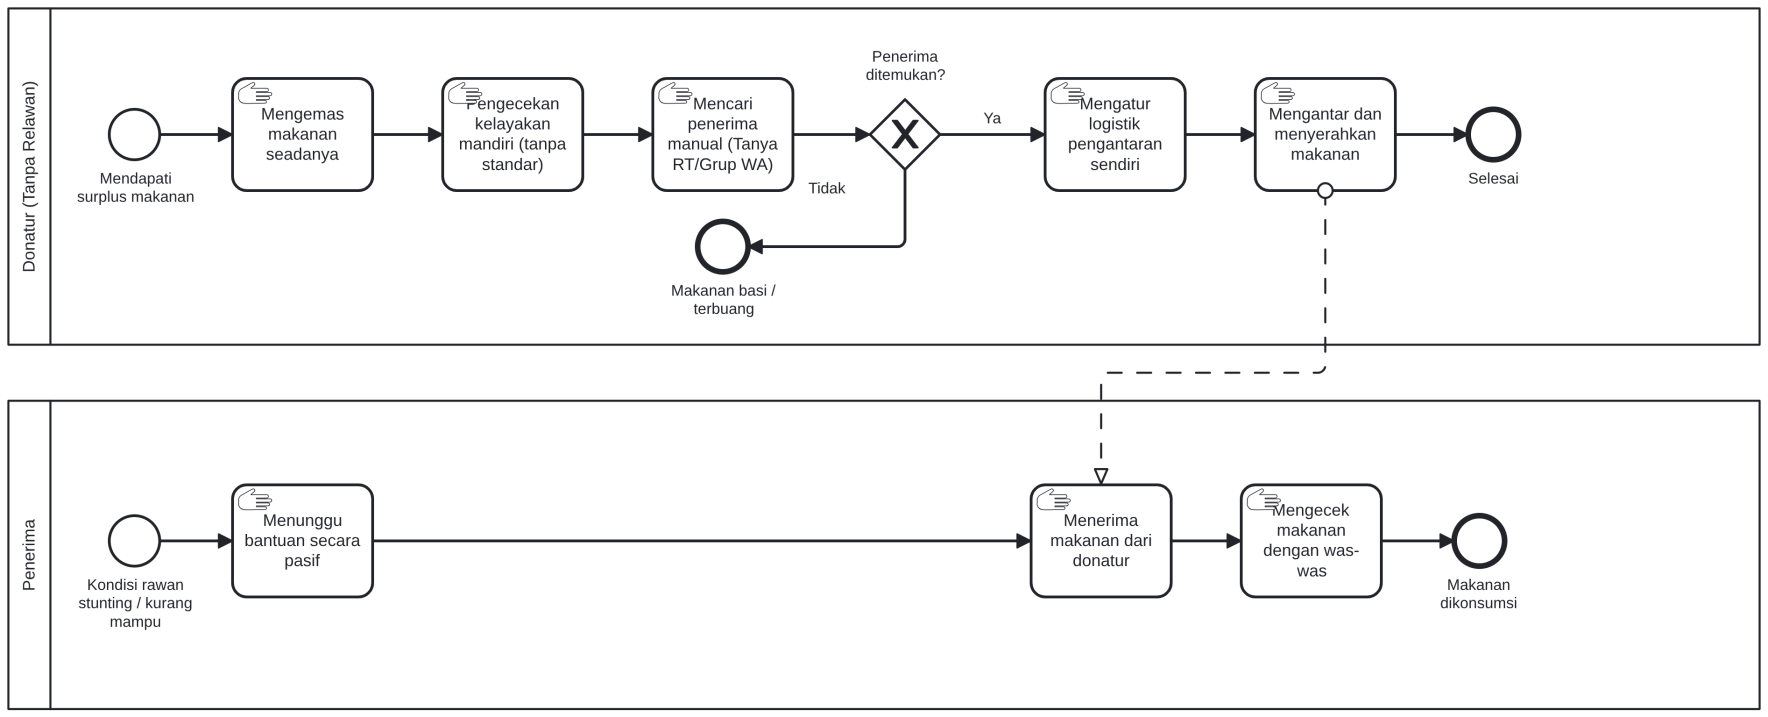
\includegraphics[width=1\linewidth]{image/bab2/as-is.png}
    \captionof{figure}{Proses Bisnis Sistem Saat Ini (BPMN As-Is)}
    \label{fig:bpmnAsIs}
    \vfill
\end{landscape}

\newpage

% Berikut adalah penjelasan detail mengenai diagram BPMN As-Is yang Diperluas (\textit{Expanded As-Is}) berdasarkan gambar tersebut.

Diagram ini membongkar realita di lapangan mengenai bagaimana proses donasi makanan sisa berjalan secara konvensional sebelum adanya intervensi sistem atau aplikasi digital. Seluruh aktivitas menggunakan \textit{Manual Task} (ikon tangan), yang menegaskan bahwa proses ini serba manual, memakan waktu, dan tidak terstandarisasi.

\subsubsection{Pool Donatur (Beban Tersentralisasi Tanpa Relawan)}
Pada sistem lama ini, Donatur memikul hampir 100\% beban operasional. Alur kerjanya adalah sebagai berikut:
\begin{itemize}
    \item Pemicu (\textit{Start Event}): Proses bermula saat donatur mendapati adanya surplus makanan (makanan berlebih yang masih layak).
    \item Persiapan Tanpa Standar: Donatur melakukan tugas "Mengemas makanan seadanya" dan "Pengecekan kelayakan mandiri (tanpa standar)". Ini adalah titik lemah pertama. Tidak ada SOP mengenai kebersihan wadah atau batas kelayakan konsumsi, murni hanya mengandalkan insting donatur.
    \item Titik Buta Informasi (\textit{Blind Spot}): Donatur kemudian "Mencari penerima manual". Aktivitas ini sangat merepotkan karena donatur harus bertanya dari mulut ke mulut (misal: ke RT setempat) atau melempar pesan di Grup WA keluarga/komunitas.
    \item Percabangan Kritis (Penerima ditemukan?):
    \begin{itemize}
        \item Jalur Gagal (Tidak): Jika pencarian memakan waktu terlalu lama atau tidak ada yang merespons, alur berbelok ke bawah menuju \textit{End Event} "Makanan basi / terbuang". Ini merepresentasikan masalah \textit{food waste} yang sering terjadi karena keterlambatan distribusi.
        \item Jalur Sukses (Ya): Jika penerima ditemukan, beban donatur belum selesai.
    \end{itemize}
    \item Kendala Logistik: Donatur harus "Mengatur logistik pengantaran sendiri". Karena ketiadaan relawan/kurir, donatur harus meluangkan waktu, tenaga, dan bensin untuk mengantar makanan tersebut.
    \item Penyelesaian: Proses diakhiri dengan "Mengantar dan menyerahkan makanan" secara langsung ke lokasi penerima.
\end{itemize}

\subsubsection{Pool Penerima (Kondisi Pasif dan Ketidakpastian)}
Di sisi seberang, alur penerima sangat pasif dan dipenuhi ketidakpastian:
\begin{itemize}
    \item Kondisi Awal: Proses penerima dipicu oleh keadaan, yaitu "Kondisi rawan stunting / kurang mampu".
    \item Sikap Pasif: Penerima hanya bisa "Menunggu bantuan secara pasif". Mereka tidak memiliki alat atau \textit{platform} untuk menyuarakan kebutuhan mereka kepada para calon donatur.
    \item Interaksi Serah Terima: Jika ada donatur yang datang, barulah penerima "Menerima makanan dari donatur" (dihubungkan oleh garis putus-putus dari \textit{pool} donatur yang merepresentasikan serah terima fisik).
    \item Isu Keamanan Pangan (\textit{Food Safety}): Setelah menerima, muncul tahap psikologis yang digambarkan sebagai "Mengecek makanan dengan was-was". Karena tidak ada jaminan atau pihak ketiga yang memvalidasi kualitas makanan tersebut, penerima mungkin merasa ragu apakah makanan tersebut masih aman dan higienis untuk dikonsumsi.
    \item Akhir Proses: Proses selesai ketika makanan akhirnya dikonsumsi.
\end{itemize}

\subsubsection{Kesimpulan Masalah (\textit{Pain Points}) pada Sistem As-Is}
Diagram ini dengan sangat jelas memetakan tiga masalah utama yang mendasari perlunya pembuatan aplikasi:
\begin{enumerate}
    \item Risiko \textit{Food Waste} yang Tinggi: Garis percabangan yang berujung pada "Makanan basi/terbuang" menunjukkan betapa rapuhnya sistem distribusi manual.
    \item Ketiadaan Dukungan Logistik: Donatur sering kali enggan mendonasikan makanannya karena malas atau tidak punya waktu untuk "Mengatur logistik pengantaran sendiri".
    \item Krisis Kepercayaan (\textit{Trust Issue}): Proses pengecekan kelayakan yang serba mandiri oleh donatur menimbulkan rasa "was-was" bagi penerima, membuktikan perlunya standarisasi dan validasi sistem (seperti pemindaian QR Code pada sistem \textit{To-Be}).
\end{enumerate}

\newpage

\begin{landscape}
    \centering
    \vfill
    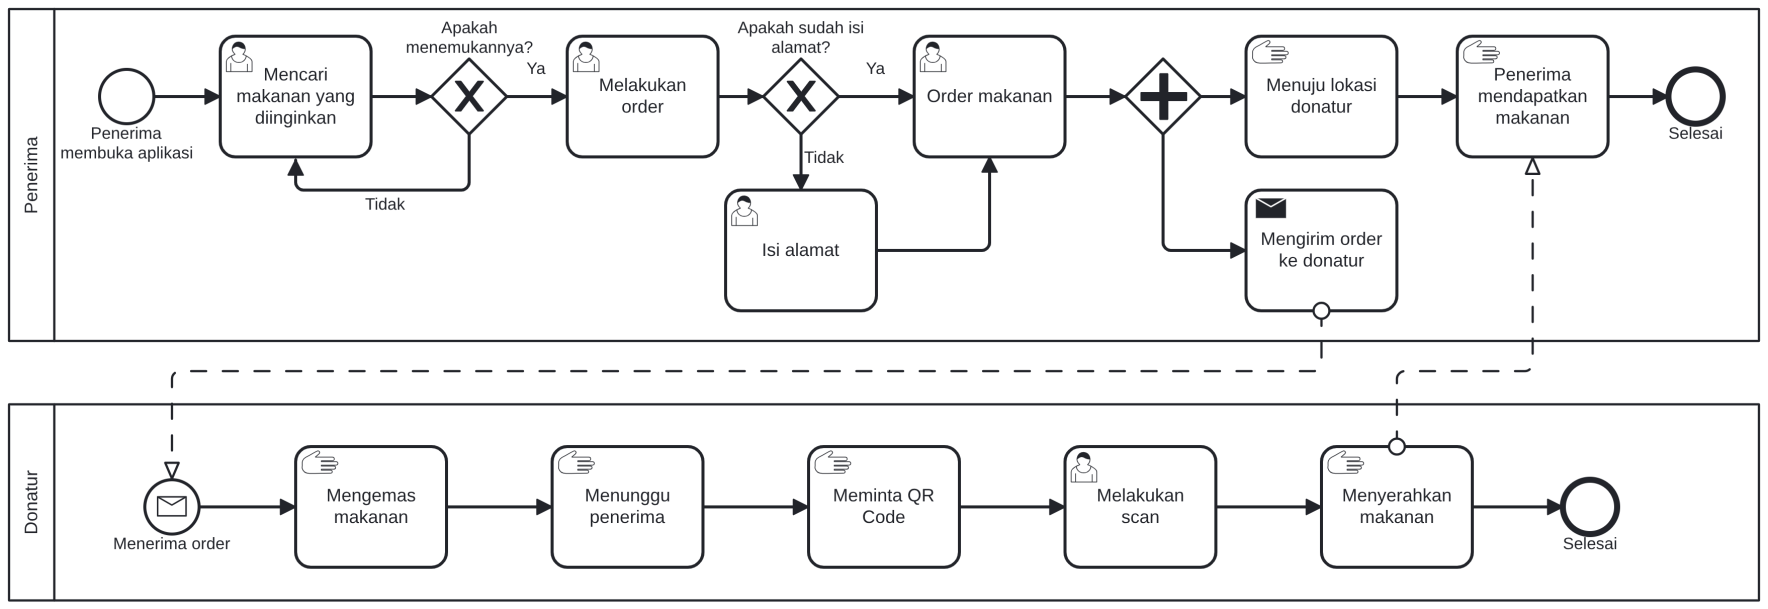
\includegraphics[width=1\linewidth]{image/bab2/to-be metode pickup.png}
    \captionof{figure}{Proses Bisnis Sistem Usulan - Metode Pickup (BPMN To-Be)}
    \label{fig:bpmnToBePickup}
    \vfill
\end{landscape}

\newpage

\subsubsection{Pool Penerima (Pusat Pemesanan dan Eksekusi Pengambilan)}
Pada metode \textit{pick-up}, aplikasi memberikan kendali penuh kepada penerima untuk bersikap proaktif. Alur detailnya adalah:
\begin{itemize}
    \item Eksplorasi dan Pemesanan Terpusat: Penerima tidak lagi hanya "menunggu bola" seperti pada sistem manual. Mereka membuka aplikasi dan langsung disajikan katalog \textit{real-time} di halaman beranda yang berisi daftar ketersediaan makanan surplus di sekitar mereka. Jika menemukan yang cocok, mereka langsung melakukan order (\textit{checkout}).
    \item Verifikasi Profil (Kelengkapan Alamat): Walaupun penerima akan mengambil sendiri, sistem tetap melakukan pengecekan (\textit{gateway}) apakah profil/alamat penerima sudah lengkap. Ini penting sebagai bentuk KYC (\textit{Know Your Customer}) untuk pendataan sistem agar \textit{user} yang bertransaksi adalah akun yang valid.
    \item Mobilisasi Mandiri: Setelah order diproses dan notifikasi terkirim ke donatur, penerima mengambil alih beban logistik. Mereka mengikuti petunjuk lokasi yang tertera di aplikasi dan bergerak secara mandiri menuju titik lokasi donatur tanpa memerlukan perantara kurir/relawan.
\end{itemize}

\subsubsection{Pool Donatur (Penyedia Donasi yang Difasilitasi)}
Sistem ini sangat meringankan beban operasional donatur. Alurnya menjadi pasif namun jauh lebih efisien:
\begin{itemize}
    \item Respons Berbasis Notifikasi (Trigger System): Donatur tidak perlu mencari siapa yang mau menerima makanannya. Sistem yang akan mencarikan. Begitu ada penerima yang melakukan order, donatur akan menerima \textit{push notification}. Notifikasi inilah yang memicu donatur untuk mulai mengemas makanan dengan layak.
    \item Menunggu Secara Pasif (Efisiensi Tenaga): Setelah mengemas, donatur cukup menunggu di tempat (rumah atau toko). Mereka bisa melanjutkan aktivitas harian mereka tanpa perlu pusing memikirkan cara mengantarkan makanan tersebut.
    \item Sistem Validasi Silang (Pemindaian QR Code): Ini adalah titik \textit{checkpoint} paling krusial dalam interaksi tatap muka. Saat penerima tiba dan mengaku sebagai pemesan, donatur wajib meminta QR Code (atau \textit{unique code}) yang tampil di layar aplikasi penerima. Donatur kemudian melakukan \textit{scan} menggunakan kameranya. Sistem akan mencocokkan data. Jika valid, serah terima fisik dilakukan, dan status order di dalam sistem otomatis berubah menjadi "Selesai".
\end{itemize}

\subsubsection{Solusi Signifikan yang Ditawarkan (Menjawab Pain Points)}
Perubahan alur ke arah digital dengan metode \textit{pick-up} ini memberikan dampak penyelesaian masalah yang terukur:
\begin{itemize}
    \item Menghapus Blind Spot Informasi Melalui Konsep "Marketplace": Sistem menjembatani informasi yang sebelumnya terputus. Donatur tidak perlu lagi menelepon atau bertanya di grup-grup komunitas. Ketersediaan makanan langsung terekspos kepada audiens yang tepat (penerima terdaftar), mempercepat proses \textit{matchmaking} antara makanan sisa dan pihak yang lapar.
    \item Memotong Rantai Logistik yang Menghambat: Pada sistem lama, tingginya angka \textit{food waste} sering kali terjadi karena donatur sibuk dan tidak ada yang bisa mengantarkan makanan. Dengan sistem \textit{pick-up}, tanggung jawab pergerakan logistik dialihkan kepada pihak yang memang membutuhkan makanan tersebut (penerima). Ini memastikan makanan lebih cepat diselamatkan selagi masih layak konsumsi.
    \item Peningkatan Keamanan, Validitas, dan Rekam Jejak (Traceability):
    \begin{itemize}
        \item Anti-Salah Sasaran: Pemindaian QR Code mengeliminasi risiko penipuan di lapangan. Donatur memiliki jaminan kepastian bahwa orang yang mengambil makanan adalah benar-benar pengguna terdaftar yang melakukan order.
        \item Digital Audit Trail: Setiap kali QR code dipindai dan makanan diserahkan, sistem mencatat waktu, lokasi, dan aktor yang terlibat ke dalam basis data. Ini menghasilkan riwayat transaksi yang transparan, memberikan rasa aman bagi kedua belah pihak.
    \end{itemize}
\end{itemize}

\newpage

\begin{landscape}
    \centering
    \vfill
    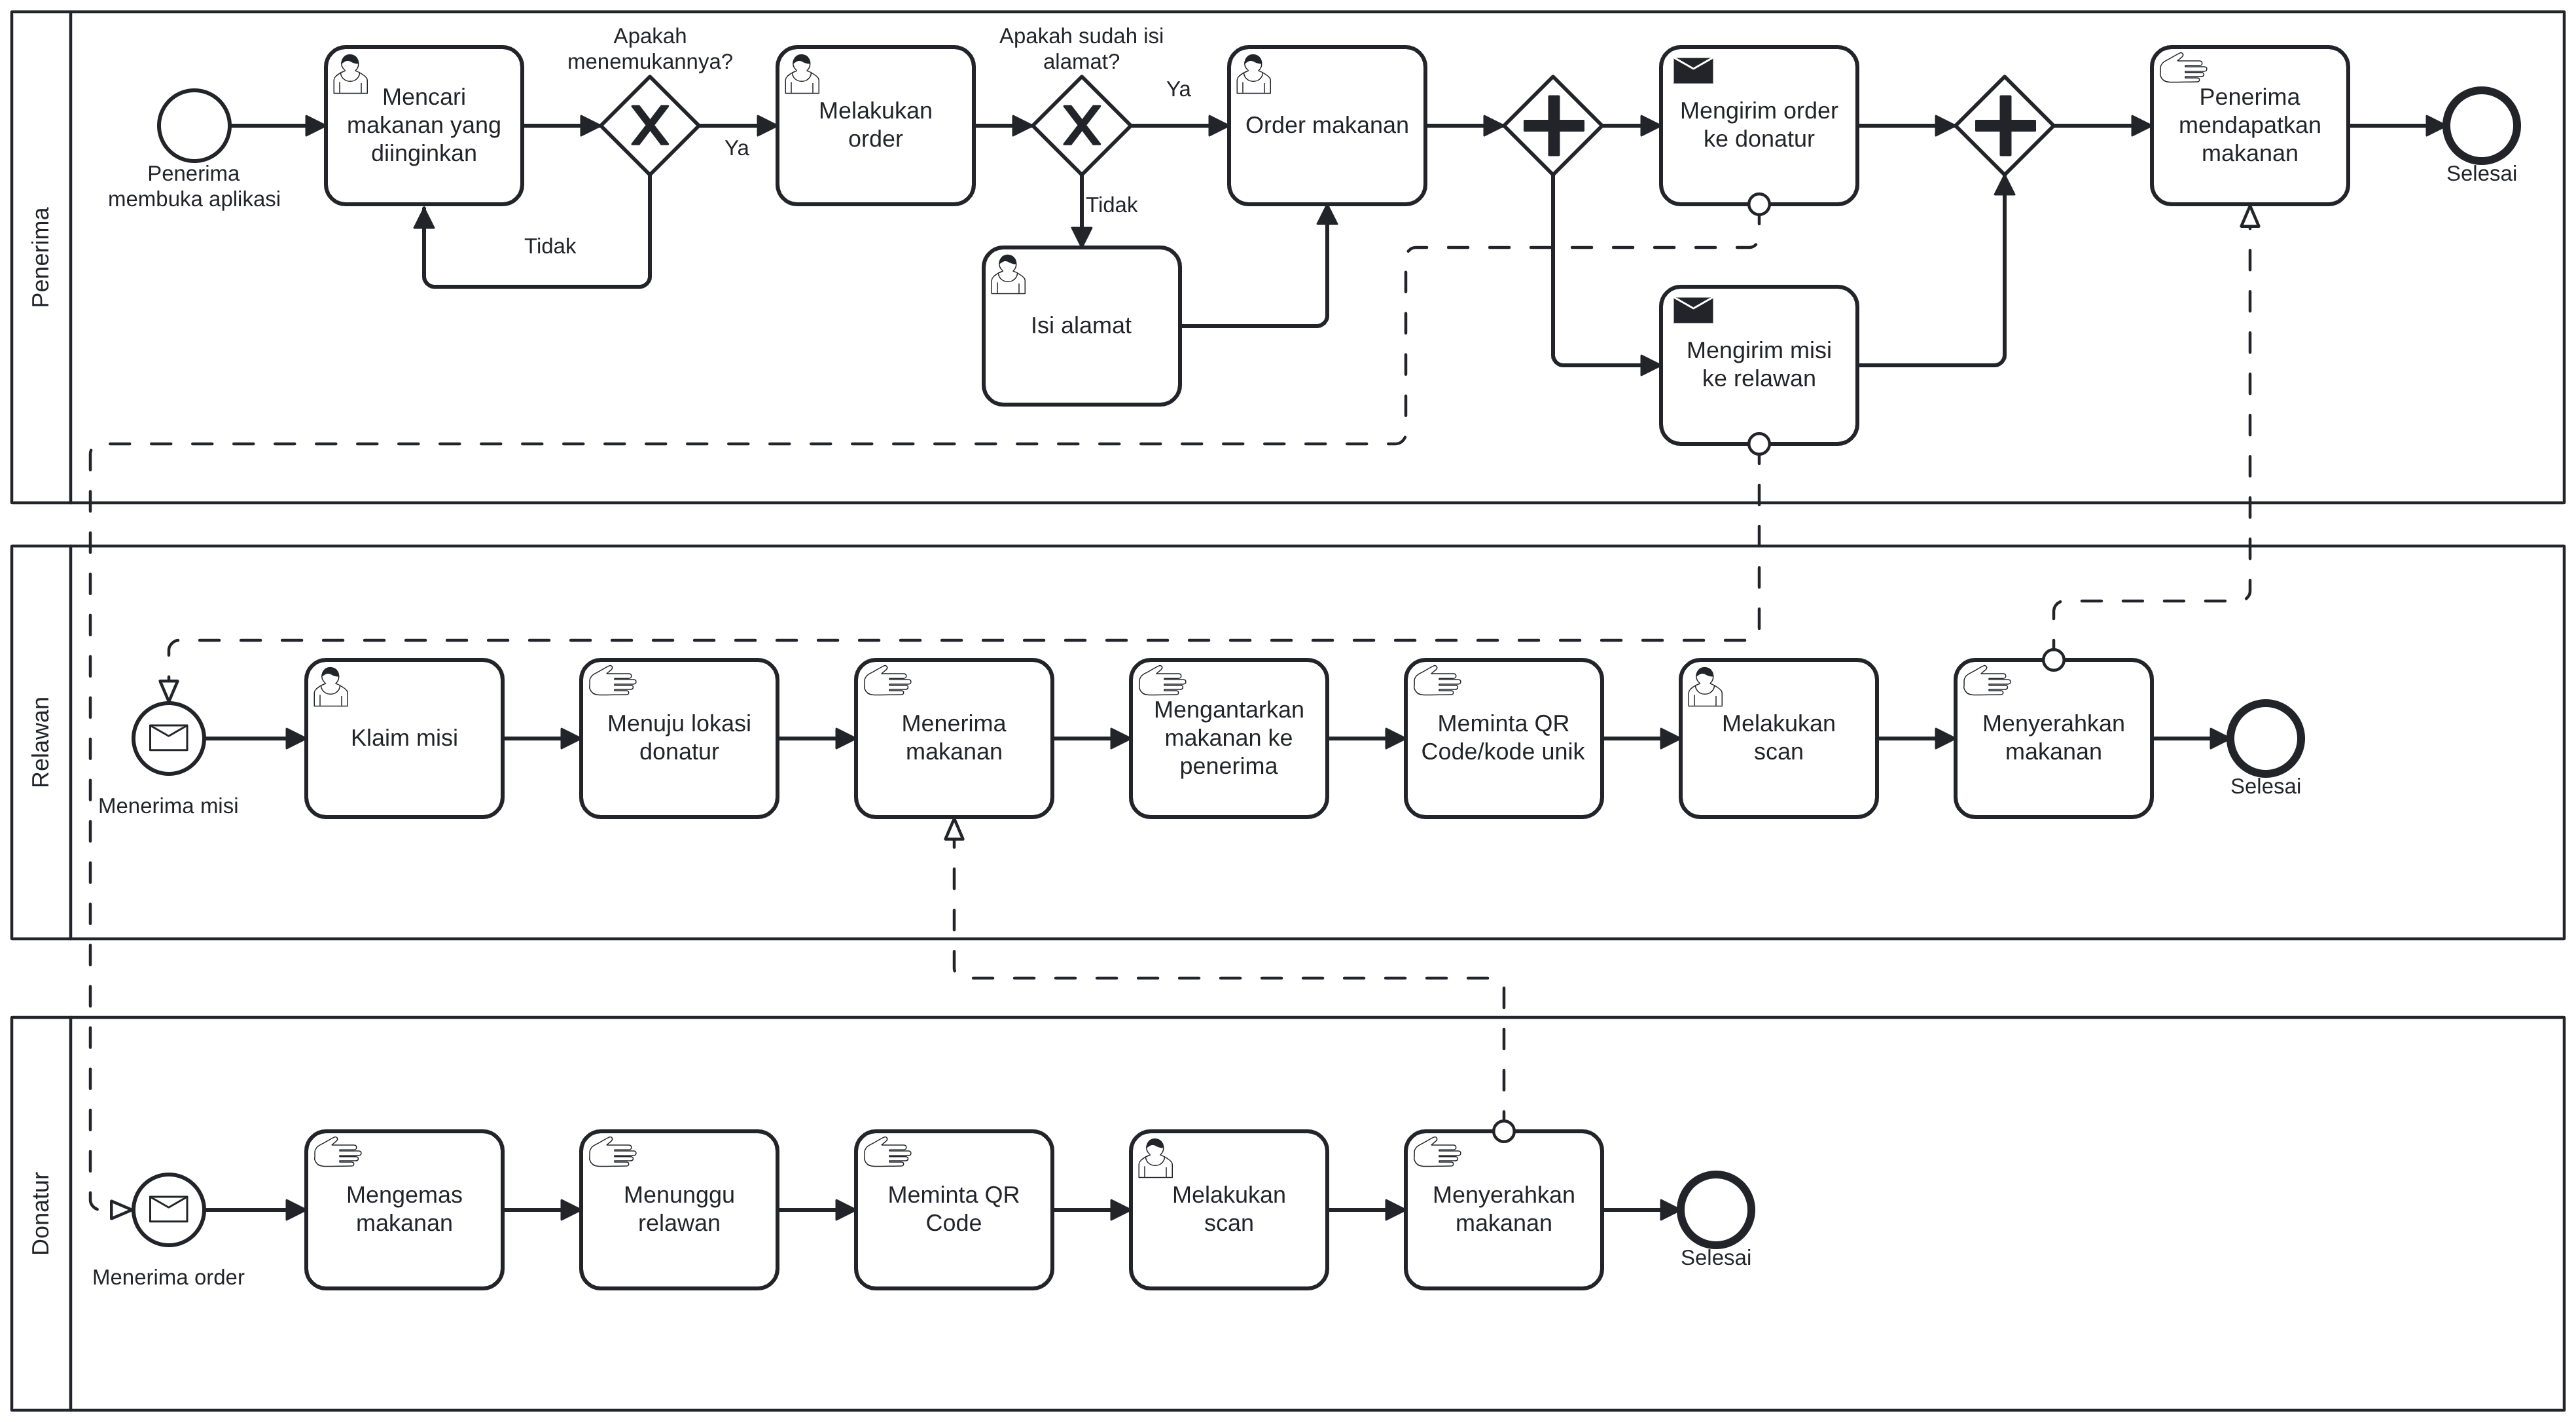
\includegraphics[width=1\linewidth]{image/bab2/to-be metode diantar.png}
    \captionof{figure}{Proses Bisnis Sistem Usulan - Metode Diantar (BPMN To-Be)}
    \label{fig:bpmnToBeDiantar}
    \vfill
\end{landscape}

\newpage

Skenario ini merupakan solusi komprehensif yang melibatkan tiga aktor sekaligus: Penerima, Donatur, dan kehadiran entitas baru yaitu Relawan. Relawan bertindak sebagai pahlawan logistik yang menjembatani donatur dan penerima.

\subsubsection{Pool Penerima (Pemesan \& Penerima Akhir)}
Pada skenario ini, penerima tetap menjadi inisiator pesanan, namun mereka hanya perlu menunggu di lokasi setelah pesanan dibuat. Alur detailnya:
\begin{itemize}
    \item Eksplorasi \& Validasi Alamat: Proses dimulai dari membuka aplikasi, mencari makanan, dan melakukan order. Sistem mengecek ketersediaan alamat; jika belum ada, pengguna wajib mengisi alamat agar relawan tahu titik pengantaran.
    \item Aksi Paralel (\textit{Parallel Gateway}): Ini adalah titik krusial (ditandai dengan ikon +). Setelah tombol "Order makanan" ditekan, sistem melakukan dua aksi pengiriman pesan (\textit{Send Task}) secara bersamaan:
    \begin{enumerate}
        \item Mengirimkan notifikasi "Order" kepada Donatur agar makanan disiapkan.
        \item Mem-\textit{broadcast} pesanan tersebut sebagai "Misi" kepada para Relawan di sekitar lokasi.
    \end{enumerate}
    \item Menunggu Kedatangan: Penerima kemudian menunggu di lokasi hingga relawan tiba untuk menyerahkan makanan. Proses selesai ketika makanan sudah di tangan penerima ("Penerima mendapatkan makanan").
\end{itemize}

\subsubsection{Pool Donatur (Penyedia Donasi)}
Alur donatur pada metode antar sangat mirip dengan metode \textit{pick-up}, namun lawan interaksinya berbeda:
\begin{itemize}
    \item Persiapan: Donatur menerima notifikasi order, lalu mulai mengemas makanan tersebut.
    \item Menunggu Relawan: Alih-alih menunggu penerima, donatur kini bersiap menunggu kedatangan Relawan yang telah mengklaim misi tersebut.
    \item Verifikasi Tahap 1 (QR Code): Ketika relawan tiba, donatur akan meminta QR Code dari relawan. Donatur kemudian melakukan \textit{scan} via aplikasi. Hal ini memastikan bahwa makanan diserahkan kepada relawan yang sah dan terdaftar di sistem, bukan sembarang orang.
    \item Serah Terima Tahap 1: Setelah validasi berhasil, donatur menyerahkan makanan kepada relawan. Proses bagi donatur pun selesai.
\end{itemize}

\subsubsection{Pool Relawan (Pahlawan Logistik)}
Ini adalah alur operasional utama bagi aktor ketiga yang bertugas menyelesaikan kendala logistik:
\begin{itemize}
    \item Penerimaan \& Klaim Misi: Relawan menerima notifikasi misi (berasal dari \textit{broadcast} sistem penerima). Jika bersedia, relawan menekan tombol "Klaim misi" di aplikasi.
    \item Fase Pengambilan (\textit{Pick-up} dari Donatur): Relawan bergerak menuju lokasi donatur. Sesampainya di sana, mereka menjalani proses verifikasi QR dari donatur, lalu "Menerima makanan".
    \item Fase Pengantaran (\textit{Delivery} ke Penerima): Relawan kemudian membawa makanan tersebut dan bergerak ("Mengantarkan makanan") menuju alamat penerima yang tertera di sistem.
    \item Verifikasi Tahap 2 (QR Code): Setibanya di lokasi tujuan, relawan tidak langsung memberikan makanan. Relawan bertugas "Meminta QR Code/kode unik" dari penerima, lalu "Melakukan scan" menggunakan aplikasinya.
    \item Serah Terima Akhir: Setelah sistem menyatakan data penerima valid, relawan menyerahkan makanan kepada penerima. Misi logistik pun selesai.
\end{itemize}

\subsubsection{Interaksi Lintas Aktor (\textit{Message Flow} - Garis Putus-putus)}
Diagram ini menunjukkan pertukaran informasi dan barang yang sangat terstruktur:
\begin{enumerate}
    \item Penerima $\rightarrow$ Donatur: Sistem mengirimkan detail order untuk disiapkan.
    \item Penerima $\rightarrow$ Relawan: Sistem menembakkan order tersebut ke \textit{pool} misi relawan.
    \item Donatur $\rightarrow$ Relawan: Interaksi fisik di mana Donatur menyerahkan kotak makanan kepada Relawan (setelah lolos \textit{scan} QR).
    \item Relawan $\rightarrow$ Penerima: Interaksi fisik akhir di mana Relawan menyerahkan kotak makanan kepada Penerima (juga setelah lolos \textit{scan} QR).
\end{enumerate}

\subsubsection{Solusi Signifikan (Perbaikan dari As-Is)}
\begin{itemize}
    \item Penyelesaian \textit{Bottleneck} Logistik: Kelemahan utama sistem lama, di mana makanan membusuk karena donatur tidak bisa mengantar dan penerima tidak bisa mengambil, terpecahkan oleh kehadiran Relawan.
    \item Keamanan Berlapis (\textit{Double-Blind Verification}): Sistem ini menerapkan keamanan ekstra ketat. Makanan melewati dua kali proses pemindaian QR Code: \textit{Donatur-ke-Relawan} dan \textit{Relawan-ke-Penerima}. Ini menjamin rantai pasok (\textit{chain of custody}) makanan tercatat sempurna di \textit{database} dari hulu ke hilir.
\end{itemize}

\newpage

\subsection{Pengalaman Pengguna}
Guna memastikan bahwa platform Food AI Rescue yang dikembangkan dapat menyelesaikan permasalahan secara akurat dan tepat sasaran, penelitian ini menerapkan pendekatan desain berpusat pada manusia (\textit{Human-Centered Design}). Pendekatan ini secara spesifik memetakan pengalaman dari target pengguna utama di lapangan, yakni pihak donatur, penerima donasi, dan relawan logistik, ketika mereka masih melakukan proses penyaluran surplus makanan secara manual atau konvensional (\textit{As-Is}). Hasil pemetaan permasalahan tersebut kemudian dituangkan ke dalam tiga artefak \textit{User Experience} (UX), meliputi \textit{User Persona}, \textit{Empathy Map}, dan \textit{User Journey Map}, yang dijabarkan sebagai berikut:

\begin{figure}[H]
    \centering
    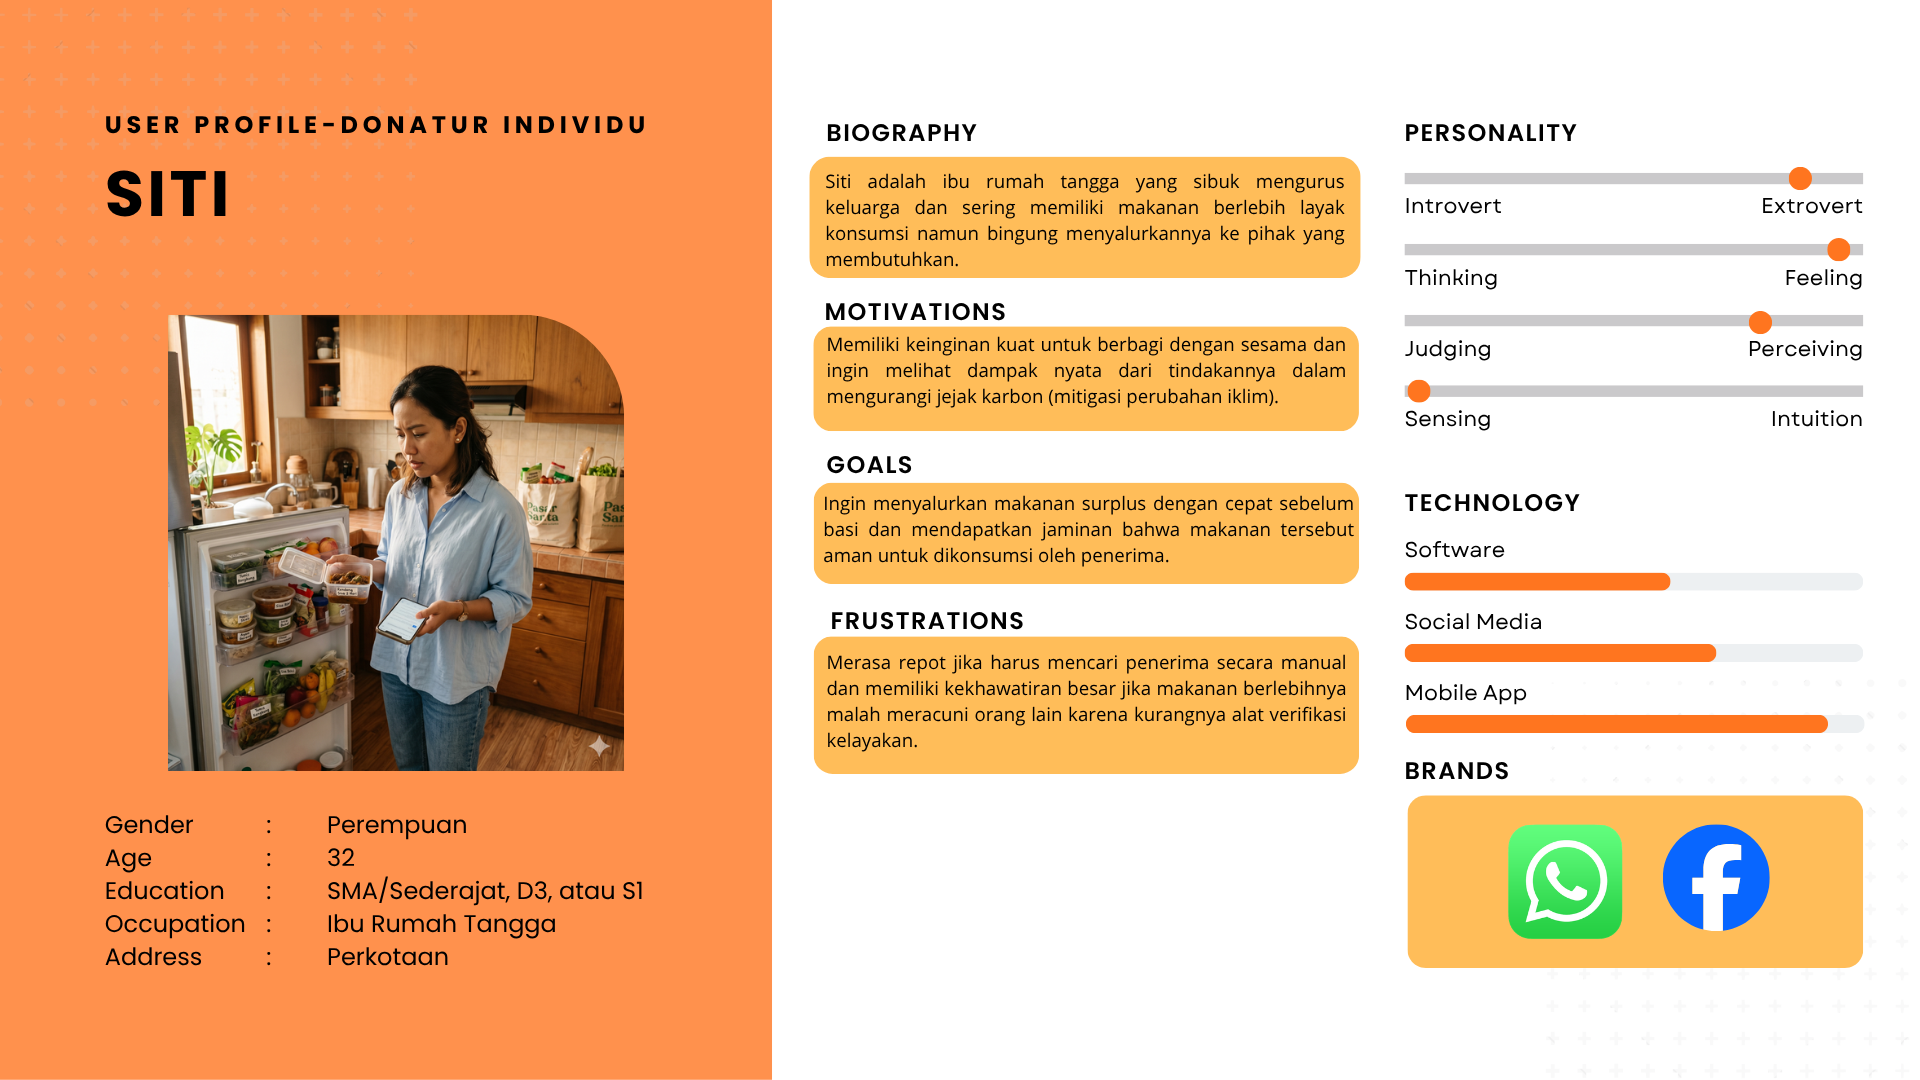
\includegraphics[width=1\textwidth]{image/bab2/segmentasi/UserPersona/Salinan dari baso arif/UP_DONATUR INDIVIDU.png}
    \caption{User Persona Donatur Individu}
    \label{fig:userPersonaDonaturIndividu}
\end{figure}

Penjelasan Profil (Siti):
Siti (32 tahun) merupakan seorang ibu rumah tangga di area perkotaan dengan jadwal padat. Ia kerap mendapati sisa bahan makanan layak konsumsi di dapur, namun kebingungan mencari cara aman untuk menyalurkannya.
\begin{itemize}
    \item Motivasi: Tergerak untuk berbagi dengan sesama dan ingin melihat dampak langsung dari usahanya dalam menekan jejak emisi karbon (mitigasi perubahan iklim).
    \item Tujuan: Mampu mendistribusikan makanan surplus dengan cepat sebelum membusuk, sekaligus memperoleh kepastian bahwa makanan tersebut higienis dan aman dikonsumsi oleh penerima.
    \item Frustrasi: Merasa sangat repot apabila harus mencari target penerima donasi secara mandiri. Terdapat kekhawatiran besar bahwa makanan berlebihnya justru dapat meracuni orang lain karena ketiadaan alat verifikasi kelayakan.
    \item Preferensi: Aplikasi \textit{mobile}, perangkat lunak (\textit{software}), media sosial, serta nilai efisiensi dalam kepedulian sosial.
\end{itemize}

% \newpage

\begin{figure}[H]
    \centering
    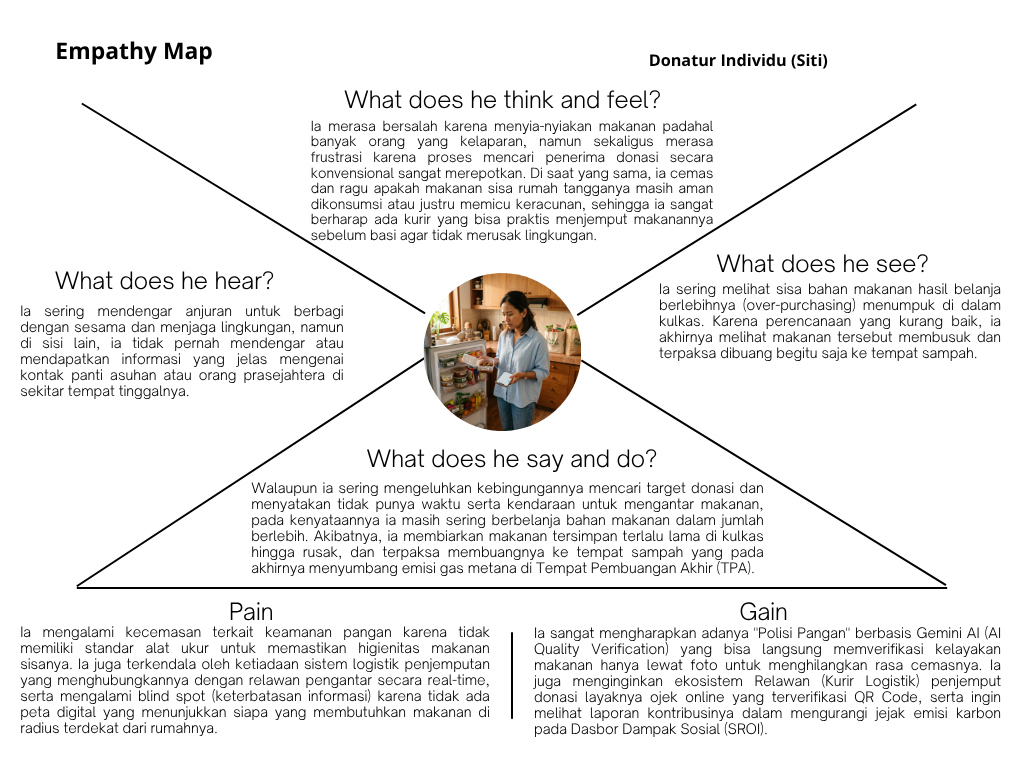
\includegraphics[width=1\textwidth]{image/bab2/segmentasi/EmpathyMap/Black and White Simple Empathy Map Brainstorm/EM_DONATUR_INDIVIDU.png}
    \caption{Empathy Map Donatur Individu}
    \label{fig:empathyMapDonaturIndividu}
\end{figure}


Penjelasan Aspek Empathy Map (Siti):
Siti adalah representasi donatur skala rumah tangga yang sering memiliki makanan berlebih, berniat kuat untuk menyumbang, namun terhalang oleh keraguan dan minimnya akses.
\begin{itemize}
    \item THINKS \& FEELS: Merasa bersalah karena menyia-nyiakan makanan di saat banyak orang kelaparan, namun sekaligus frustrasi akibat proses pencarian penerima yang merepotkan. Ia cemas apakah sisa makanannya masih aman dimakan atau justru memicu keracunan, sehingga sangat berharap ada layanan kurir penjemputan praktis sebelum makanannya membusuk dan merusak lingkungan.
    \item HEARS: Kerap mendengar anjuran untuk saling berbagi dan menjaga lingkungan, tetapi di sisi lain, ia tidak pernah mendapatkan informasi pasti atau kontak mengenai panti asuhan maupun warga prasejahtera di sekitar tempat tinggalnya.
    \item SEES: Menyaksikan langsung tumpukan sisa bahan makanan di kulkas akibat kebiasaan belanja berlebih (\textit{over-purchasing}). Karena minimnya perencanaan, ia akhirnya hanya bisa melihat makanan tersebut membusuk dan terpaksa membuangnya ke tempat sampah.
    \item SAYS \& DOES: Meskipun sering mengeluh kebingungan mencari target donasi dan menyatakan tidak punya waktu serta kendaraan untuk mengantar, pada praktiknya ia tetap membiarkan makanan tersimpan terlalu lama di kulkas. Akibatnya, makanan tersebut rusak dan dibuang ke TPA, yang pada akhirnya menyumbang emisi gas metana.
    \item PAINS: Mengalami kecemasan terkait keamanan pangan karena ketiadaan alat ukur higienitas. Ia juga terhambat oleh ketiadaan sistem logistik penjemputan (\textit{pick-up}) \textit{real-time}, serta mengalami \textit{blind spot} (keterbatasan informasi) mengenai lokasi pihak yang membutuhkan di radius terdekatnya.
    \item GAINS: Sangat mendambakan kehadiran "Polisi Pangan" berbasis AI yang mampu memvalidasi kelayakan makanan hanya melalui foto. Ia juga menginginkan ekosistem Relawan Kurir layaknya ojek \textit{online} yang terverifikasi QR Code, serta Dasbor SROI untuk melihat laporan kontribusinya dalam mengurangi jejak karbon.
\end{itemize}

% \newpage

\begin{figure}[H]
    \centering
    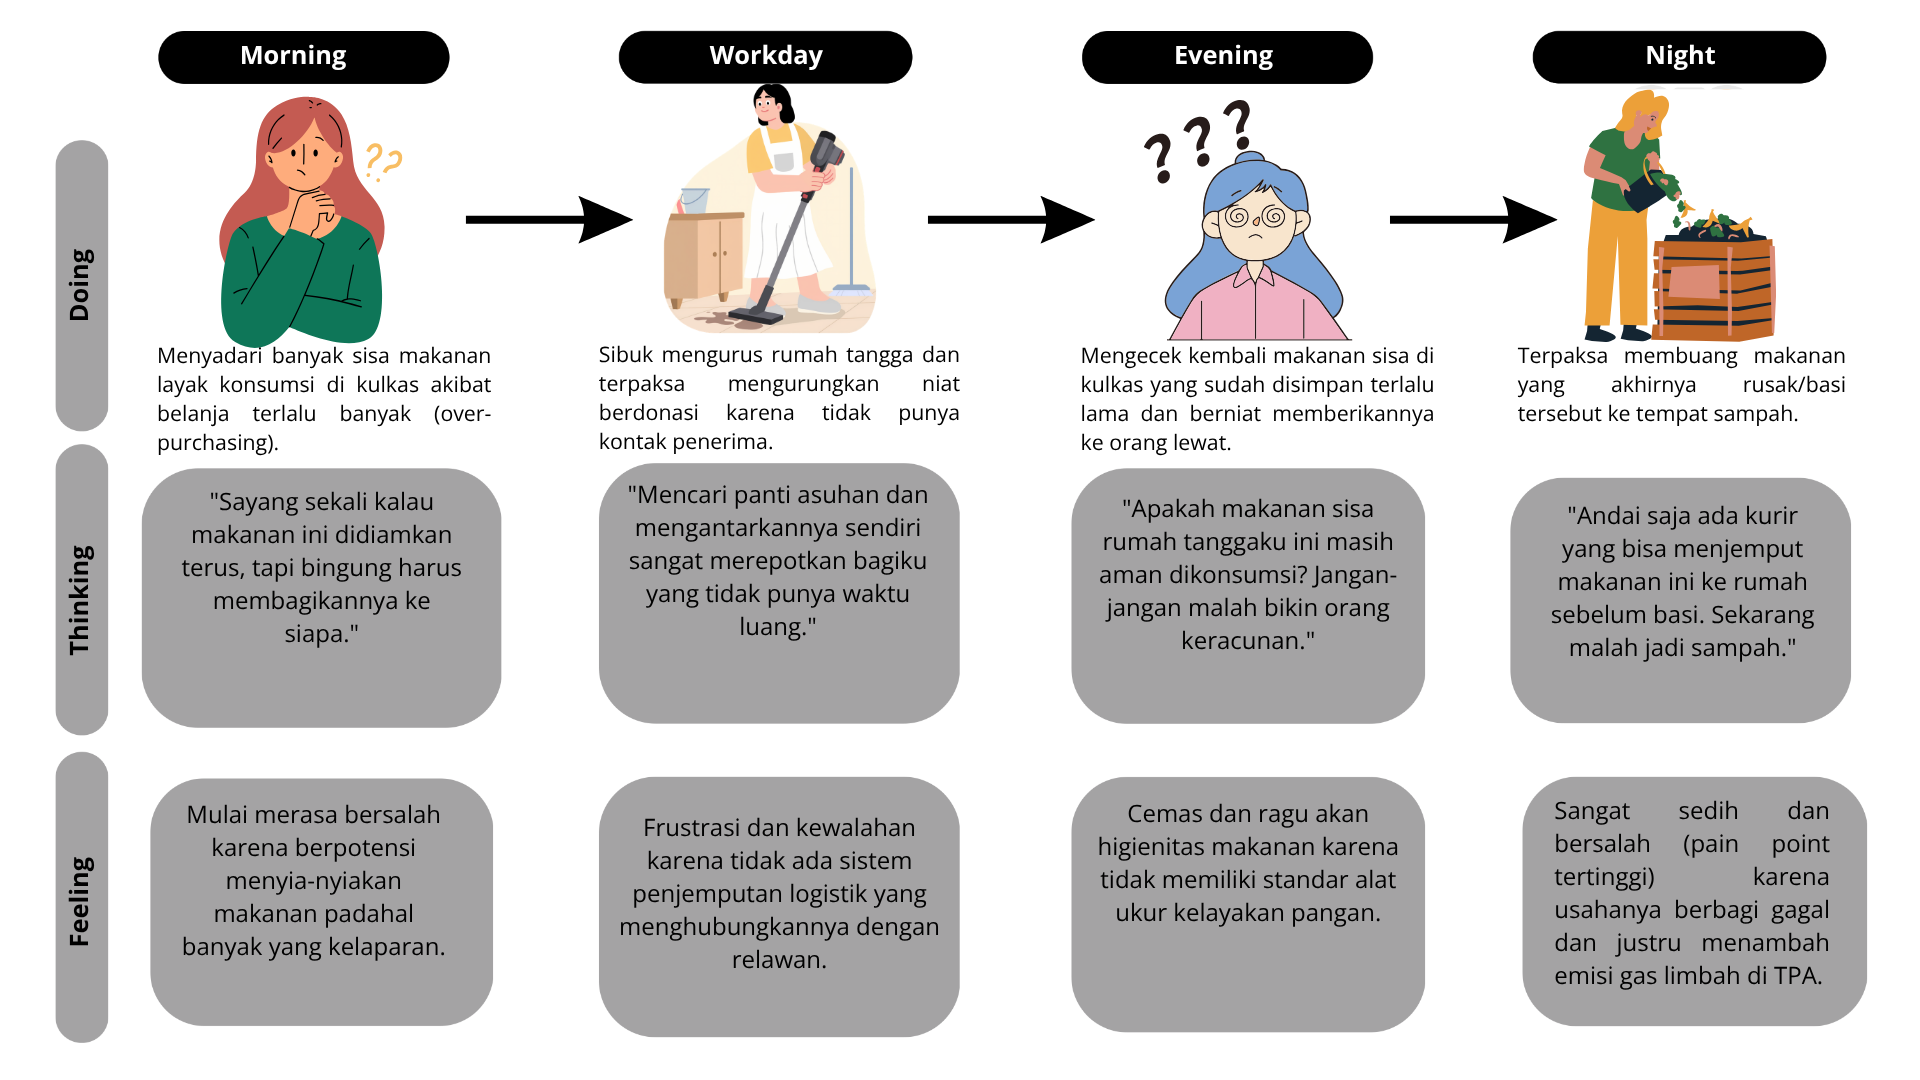
\includegraphics[width=0.99\textwidth]{image/bab2/segmentasi/CustomerJourneyMap/Salinan dari Template Journey Map/CJM_DONATUR_INDIVIDU.png}
    \caption{Customer Journey Map Donatur Individu}
    \label{fig:customerJourneyMapDonaturIndividu}
\end{figure}

Penjelasan Fase Customer Journey Map (Siti): \\
\textit{Fase perjalanan: Penumpukan Makanan $\rightarrow$ Keterbatasan Akses $\rightarrow$ Krisis Kepercayaan $\rightarrow$ Pembuangan \& Penyesalan}
\begin{description}
    \item[Penumpukan Makanan (Pagi):] Siti menyadari adanya banyak sisa makanan yang masih layak konsumsi di dalam kulkas akibat belanja berlebihan. Ia mulai didera rasa bersalah karena berpotensi menyia-nyiakan makanan tersebut, namun kebingungan harus menyalurkannya ke mana. Peluang Solusi (FAR): Fitur rekomendasi resep masakan berbasis AI untuk memanfaatkan bahan sisa.
    \item[Keterbatasan Akses (Siang):] Di tengah kesibukannya mengurus rumah tangga, Siti terpaksa mengurungkan niat untuk berdonasi karena ia tidak memiliki kontak penerima dan merasa sangat merepotkan jika harus mencari sekaligus mengantarkannya sendiri tanpa waktu luang. Peluang Solusi (FAR): Sistem panggilan Relawan Kurir secara instan untuk penjemputan langsung ke rumah.
    \item[Krisis Kepercayaan (Sore):] Ia kembali mengecek makanan tersebut dan berniat membagikannya ke orang lewat, namun tiba-tiba merasa cemas dan ragu. Tanpa adanya standar alat ukur, ia takut makanannya sudah tidak higienis dan malah menyebabkan keracunan. Peluang Solusi (FAR): Verifikasi AI \textit{Quality Verification} ("Polisi Pangan") untuk memastikan keamanan pangan secara instan.
    \item[Pembuangan \& Penyesalan (Malam):] Pada akhirnya, Siti terpaksa membuang makanan yang sudah terlanjur basi tersebut ke tempat sampah. Ia merasa sangat sedih dan bersalah (\textit{Pain Point Tertinggi}) karena usahanya untuk berbagi berujung gagal, dan ia justru berkontribusi menambah emisi gas limbah di TPA. Peluang Solusi (FAR): Dasbor SROI Pribadi yang memotivasi pengguna dengan menampilkan total porsi terselamatkan dan emisi yang dicegah.
\end{description}

% \clearpage

\begin{figure}[H]
    \centering
    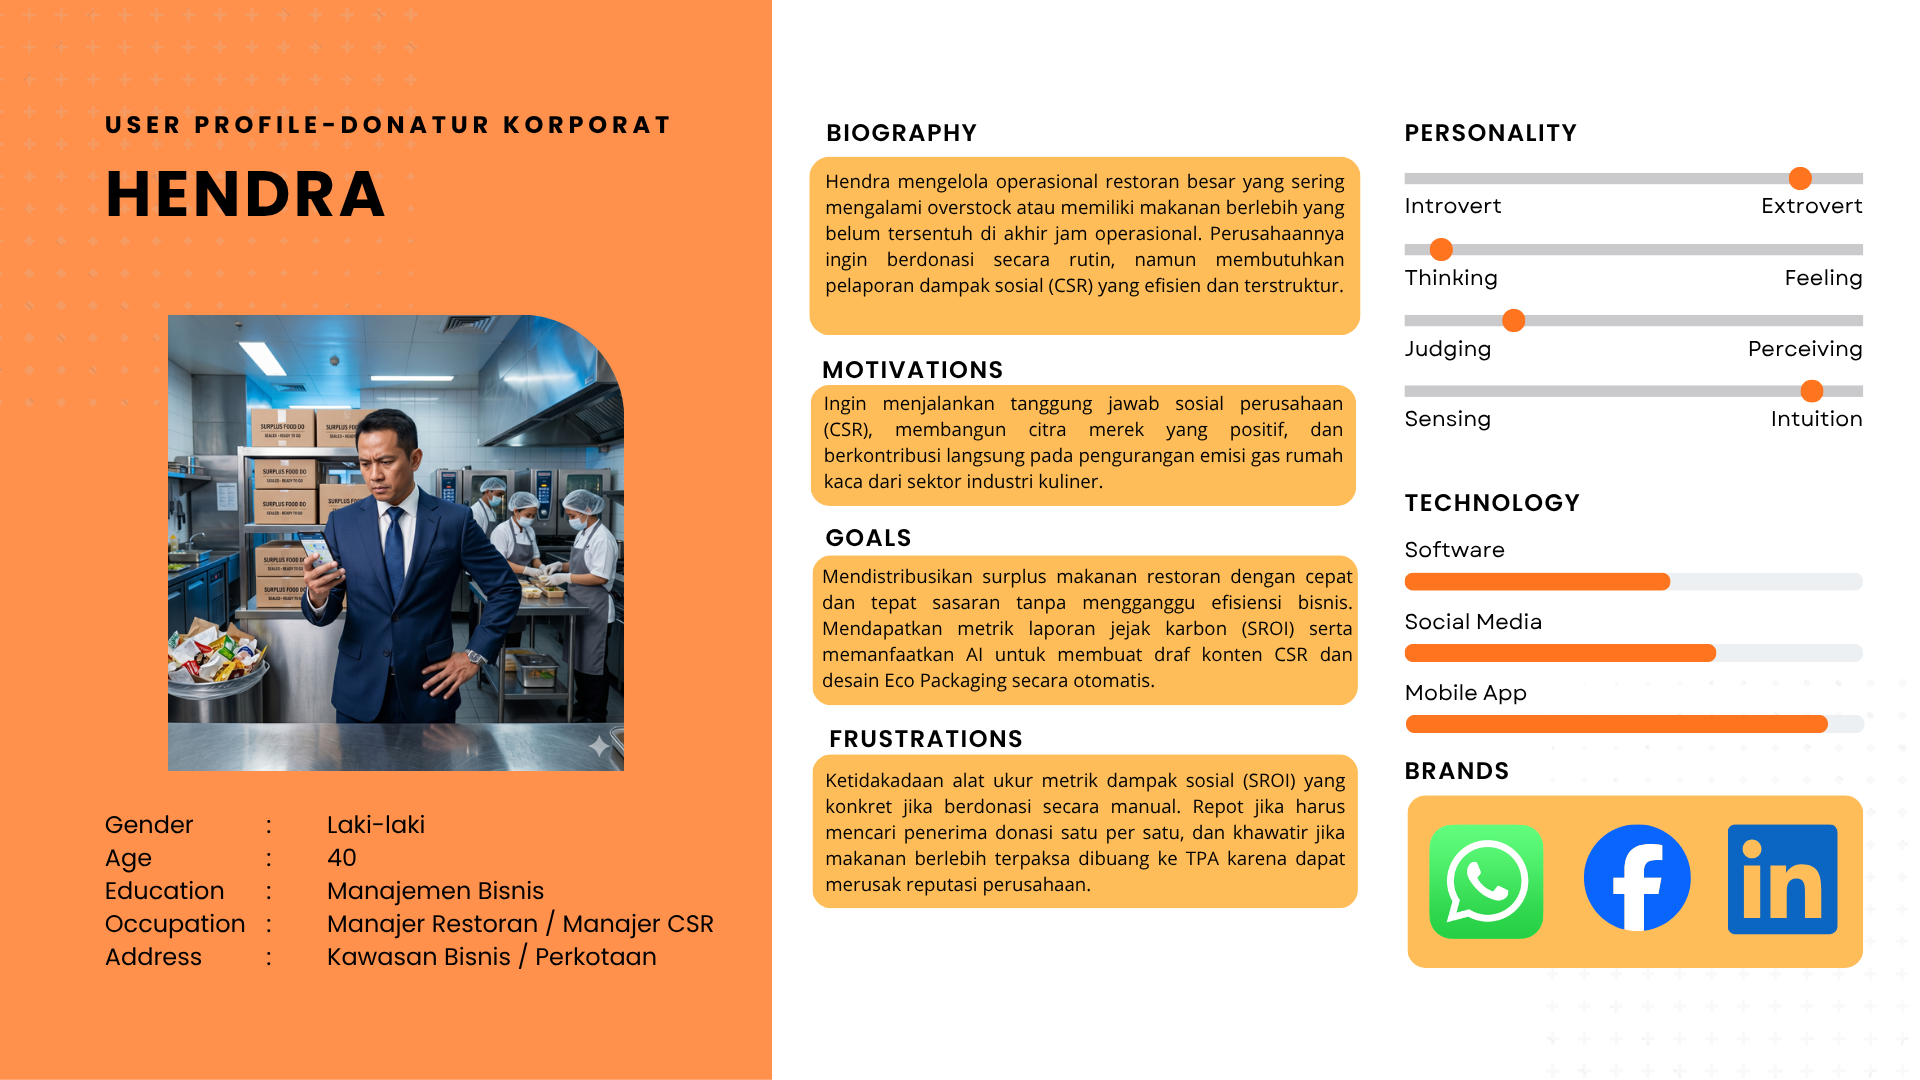
\includegraphics[width=1\textwidth]{image/bab2/segmentasi/UserPersona/Salinan dari baso arif/UP_DONATUR KORPORAT.png}
    \caption{User Persona Donatur Korporat}
    \label{fig:userPersonaDonaturKorporat}
\end{figure}

Penjelasan Profil (Hendra):
Hendra (40 tahun) menjabat sebagai manajer restoran sekaligus penanggung jawab CSR yang berhadapan dengan masalah \textit{overstock} makanan layak konsumsi di penghujung jam operasional. Perusahaannya memiliki inisiatif untuk rutin berdonasi, namun sangat membutuhkan sistem pelaporan dampak sosial yang efisien dan terstruktur.
\begin{itemize}
    \item Motivasi: Berkomitmen menjalankan kewajiban CSR perusahaan, meningkatkan citra positif merek, serta berkontribusi nyata dalam menekan emisi gas rumah kaca dari sektor industri kuliner.
    \item Tujuan: Mendistribusikan surplus makanan restoran secara cepat dan tepat sasaran tanpa mengorbankan efisiensi operasional bisnis. Ia juga ingin mendapatkan metrik Laporan Jejak Karbon (SROI) serta memanfaatkan teknologi AI untuk mengotomatisasi penyusunan konten CSR.
    \item Frustrasi: Ketidakadaan alat ukur metrik dampak sosial (SROI) yang valid saat berdonasi manual. Ia merasa repot jika harus mencari penerima satu per satu, dan sangat khawatir jika surplus makanan terpaksa dibuang ke TPA karena dapat merusak reputasi perusahaan.
    \item Preferensi: Aplikasi \textit{mobile}, perangkat lunak (\textit{software}), integrasi AI, media sosial, dan metrik bisnis yang selaras dengan kepedulian lingkungan.
\end{itemize}


\begin{figure}[H]
    \centering
    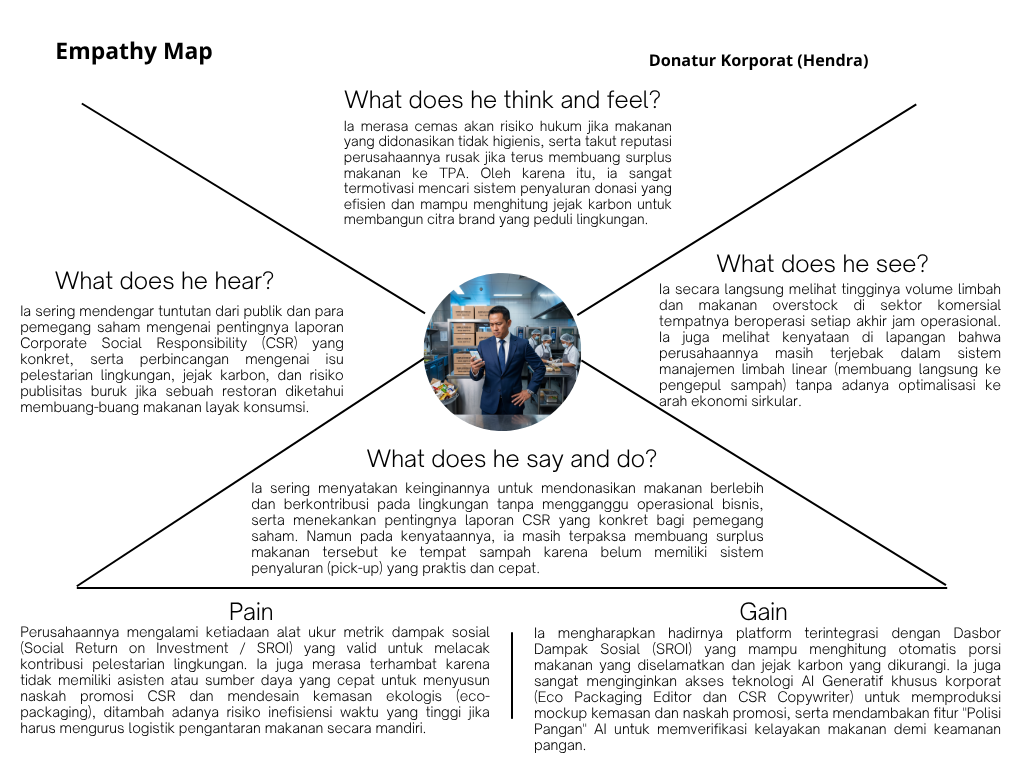
\includegraphics[width=1\textwidth]{image/bab2/segmentasi/EmpathyMap/Black and White Simple Empathy Map Brainstorm/EM_DONATUR_KORPORAT.png}
    \caption{Empathy Map Donatur Korporat}
    \label{fig:empathyMapDonaturKorporat}
\end{figure}

Penjelasan Aspek Empathy Map (Hendra):
Hendra adalah manajer restoran komersial yang ingin menyalurkan surplus makanan dengan praktis, namun sangat tertekan oleh tuntutan pelaporan reputasi dan efisiensi operasional.
\begin{itemize}
    \item THINKS \& FEELS: Dirundung kecemasan terkait potensi risiko hukum apabila makanan donasi terbukti tidak higienis. Di sisi lain, ia takut reputasi bisnisnya hancur jika terus-menerus membuang surplus ke TPA. Oleh karena itu, ia sangat termotivasi mencari sistem penyaluran efisien yang mampu menghitung jejak karbon demi citra merek peduli lingkungan.
    \item HEARS: Terus-menerus mendengar desakan dari publik dan pemegang saham mengenai urgensi pelaporan CSR yang konkret. Ia juga sering mendengar perbincangan terkait isu kelestarian lingkungan, jejak karbon, serta ancaman publisitas buruk bagi restoran yang kedapatan membuang makanan layak konsumsi.
    \item SEES: Menghadapi langsung realita tingginya volume limbah dan makanan \textit{overstock} di sektor komersial setiap kali jam operasional berakhir. Ia melihat kenyataan di lapangan bahwa perusahaannya masih terbelenggu dalam sistem manajemen limbah linear (membuang langsung ke pengepul sampah) tanpa optimalisasi ke arah ekonomi sirkular.
    \item SAYS \& DOES: Kerap mengutarakan niat mendonasikan makanan berlebih tanpa mengganggu ritme operasional bisnis, serta menekankan pentingnya laporan CSR yang nyata bagi investor. Namun pada kenyataannya, ketiadaan sistem penyaluran (\textit{pick-up}) yang cepat memaksanya untuk terus membuang surplus makanan tersebut ke tempat sampah.
    \item PAINS: Perusahaannya mengalami krisis ketiadaan alat ukur metrik dampak sosial (SROI) yang valid untuk melacak kontribusi pelestarian lingkungan. Ia juga merasa terhambat karena tidak memiliki asisten cepat untuk menyusun naskah promosi CSR dan desain kemasan ekologis, ditambah tingginya risiko inefisiensi waktu jika mengurus logistik pengantaran sendiri.
    \item GAINS: Sangat menantikan platform terintegrasi dengan Dasbor Dampak Sosial (SROI) yang mampu menghitung otomatis porsi makanan terselamatkan dan jejak karbon yang dikurangi. Ia mendambakan fitur AI Generatif khusus korporat (\textit{Eco Packaging Editor} dan \textit{CSR Copywriter}) untuk memproduksi \textit{mockup} promosi, serta "Polisi Pangan" AI untuk memvalidasi kelayakan demi keamanan pangan.
\end{itemize}

\begin{figure}[H]
    \centering
    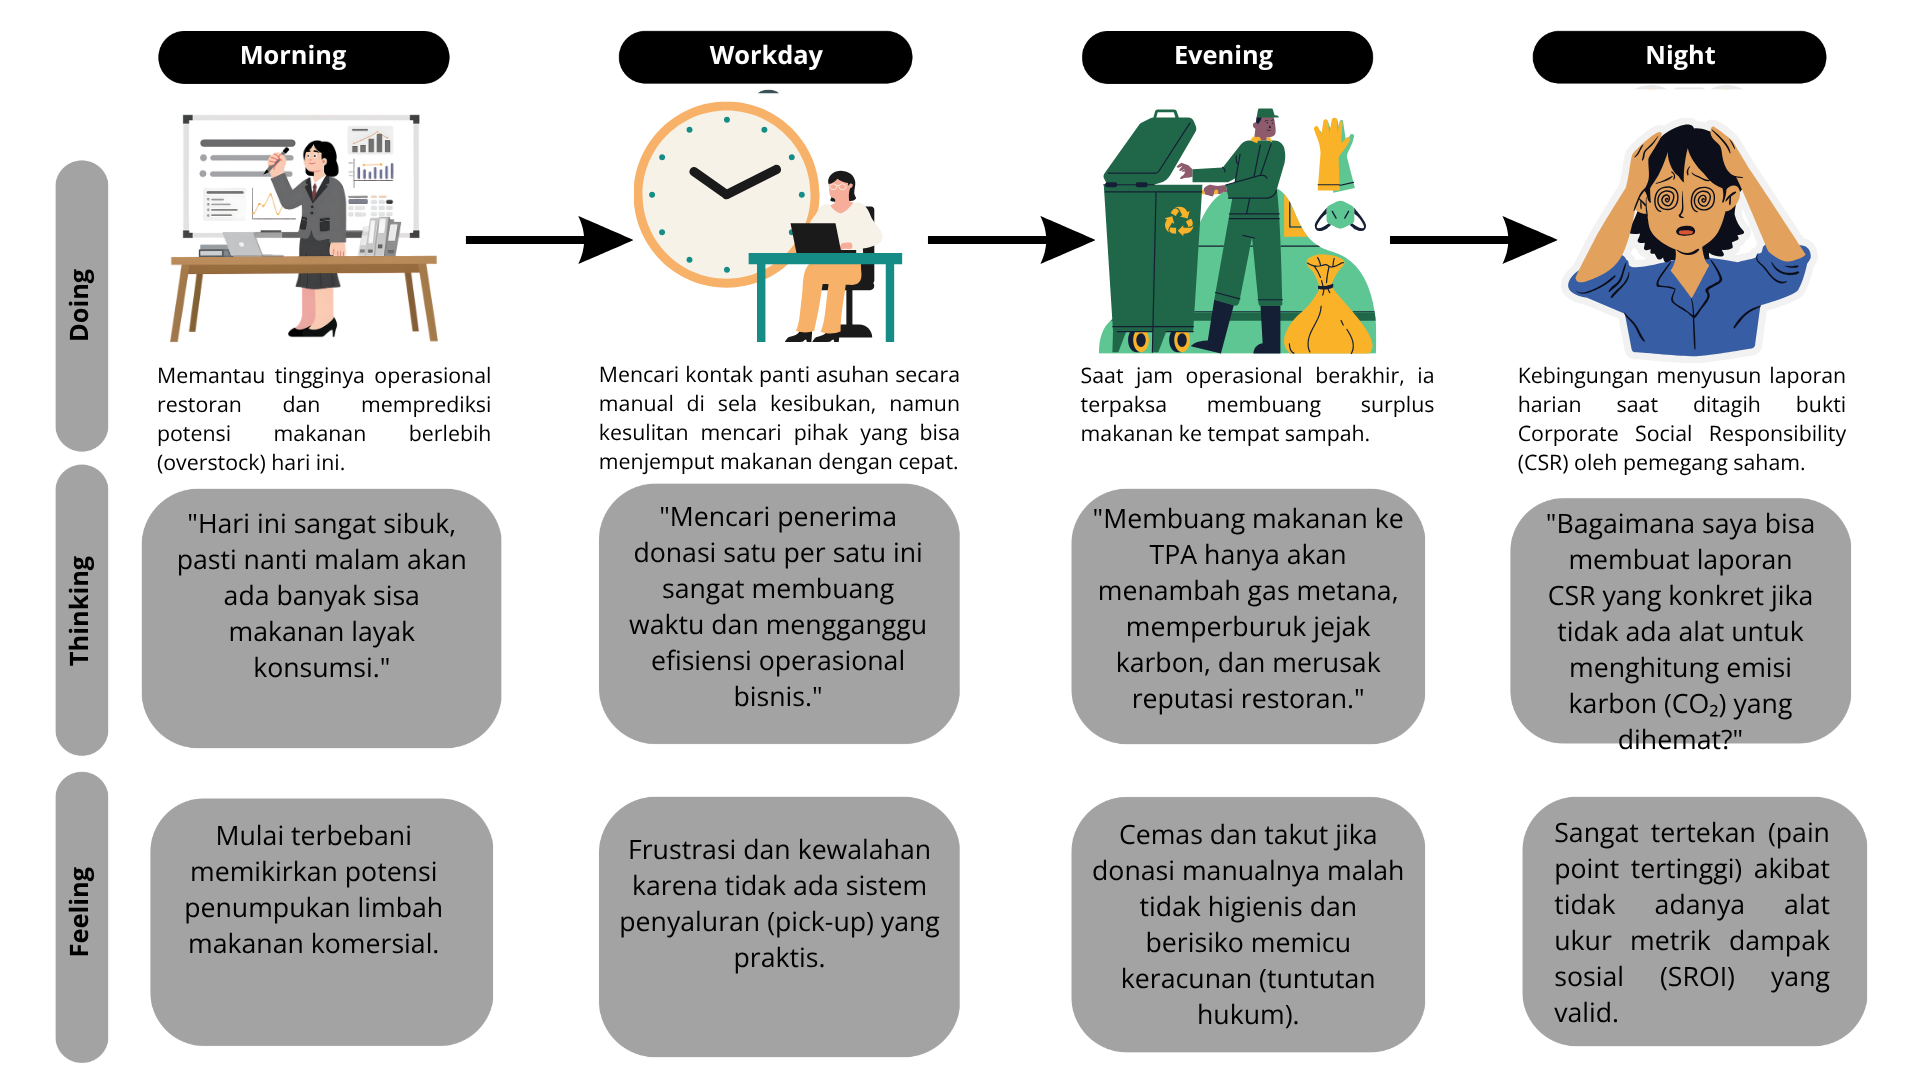
\includegraphics[width=0.99\textwidth]{image/bab2/segmentasi/CustomerJourneyMap/Salinan dari Template Journey Map/CJM_DONATUR_KORPORAT.png}
    \caption{Customer Journey Map Donatur Korporat}
    \label{fig:customerJourneyMapDonaturKorporat}
\end{figure}

Penjelasan Fase Customer Journey Map (Hendra): \\
\textit{Fase perjalanan: Prediksi Operasional $\rightarrow$ Pencarian Penerima Manual $\rightarrow$ Pembuangan Surplus $\rightarrow$ Kebingungan Pelaporan}
\begin{description}
    \item[Prediksi Operasional (Pagi):] Hendra mengawali hari dengan memantau padatnya operasional restoran. Ia sudah bisa memprediksi dan mulai terbebani memikirkan potensi penumpukan limbah makanan komersial (\textit{overstock}) di hari itu. Peluang Solusi (FAR): Login peran khusus korporat (RBAC) dengan dasbor prediksi volume surplus makanan untuk persiapan alokasi dini.
    \item[Pencarian Penerima Manual (Siang):] Di sela-sela kesibukan kerja, Hendra mencoba mencari kontak panti asuhan secara manual. Ia merasa frustrasi dan kewalahan karena sangat kesulitan menemukan pihak yang bisa menjemput makanan dengan cepat tanpa mengganggu efisiensi operasional bisnis. Peluang Solusi (FAR): Sistem otomatis (\textit{Missions Board}) yang menghubungkan tugas penjemputan logistik langsung ke Relawan Kurir.
    \item[Pembuangan Surplus (Sore):] Saat jam operasional berakhir, Hendra dilanda cemas dan takut mendonasikan makanannya secara manual. Tanpa standar higienitas, ia takut donasinya malah berisiko memicu keracunan dan tuntutan hukum. Akibatnya, ia terpaksa membuang surplus makanan tersebut ke TPA. Peluang Solusi (FAR): Fitur Wajib Pindai (\textit{Mandatory Scan}) QR Code dan validasi "Polisi Pangan" sebagai bukti serah terima yang aman secara hukum.
    \item[Kebingungan Pelaporan (Malam):] Hendra merasa sangat tertekan (\textit{Pain Point Tertinggi}) saat ditagih bukti pelaporan CSR oleh para pemegang saham. Ia kebingungan menyusun laporan harian yang konkret karena tidak adanya alat ukur untuk menghitung emisi karbon yang dihemat. Peluang Solusi (FAR): Dasbor SROI Korporat yang menyajikan angka penurunan emisi secara otomatis, terintegrasi dengan AI \textit{CSR Copywriter} untuk membuat laporan harian.
\end{description}

% \clearpage

\begin{figure}[H]
    \centering
    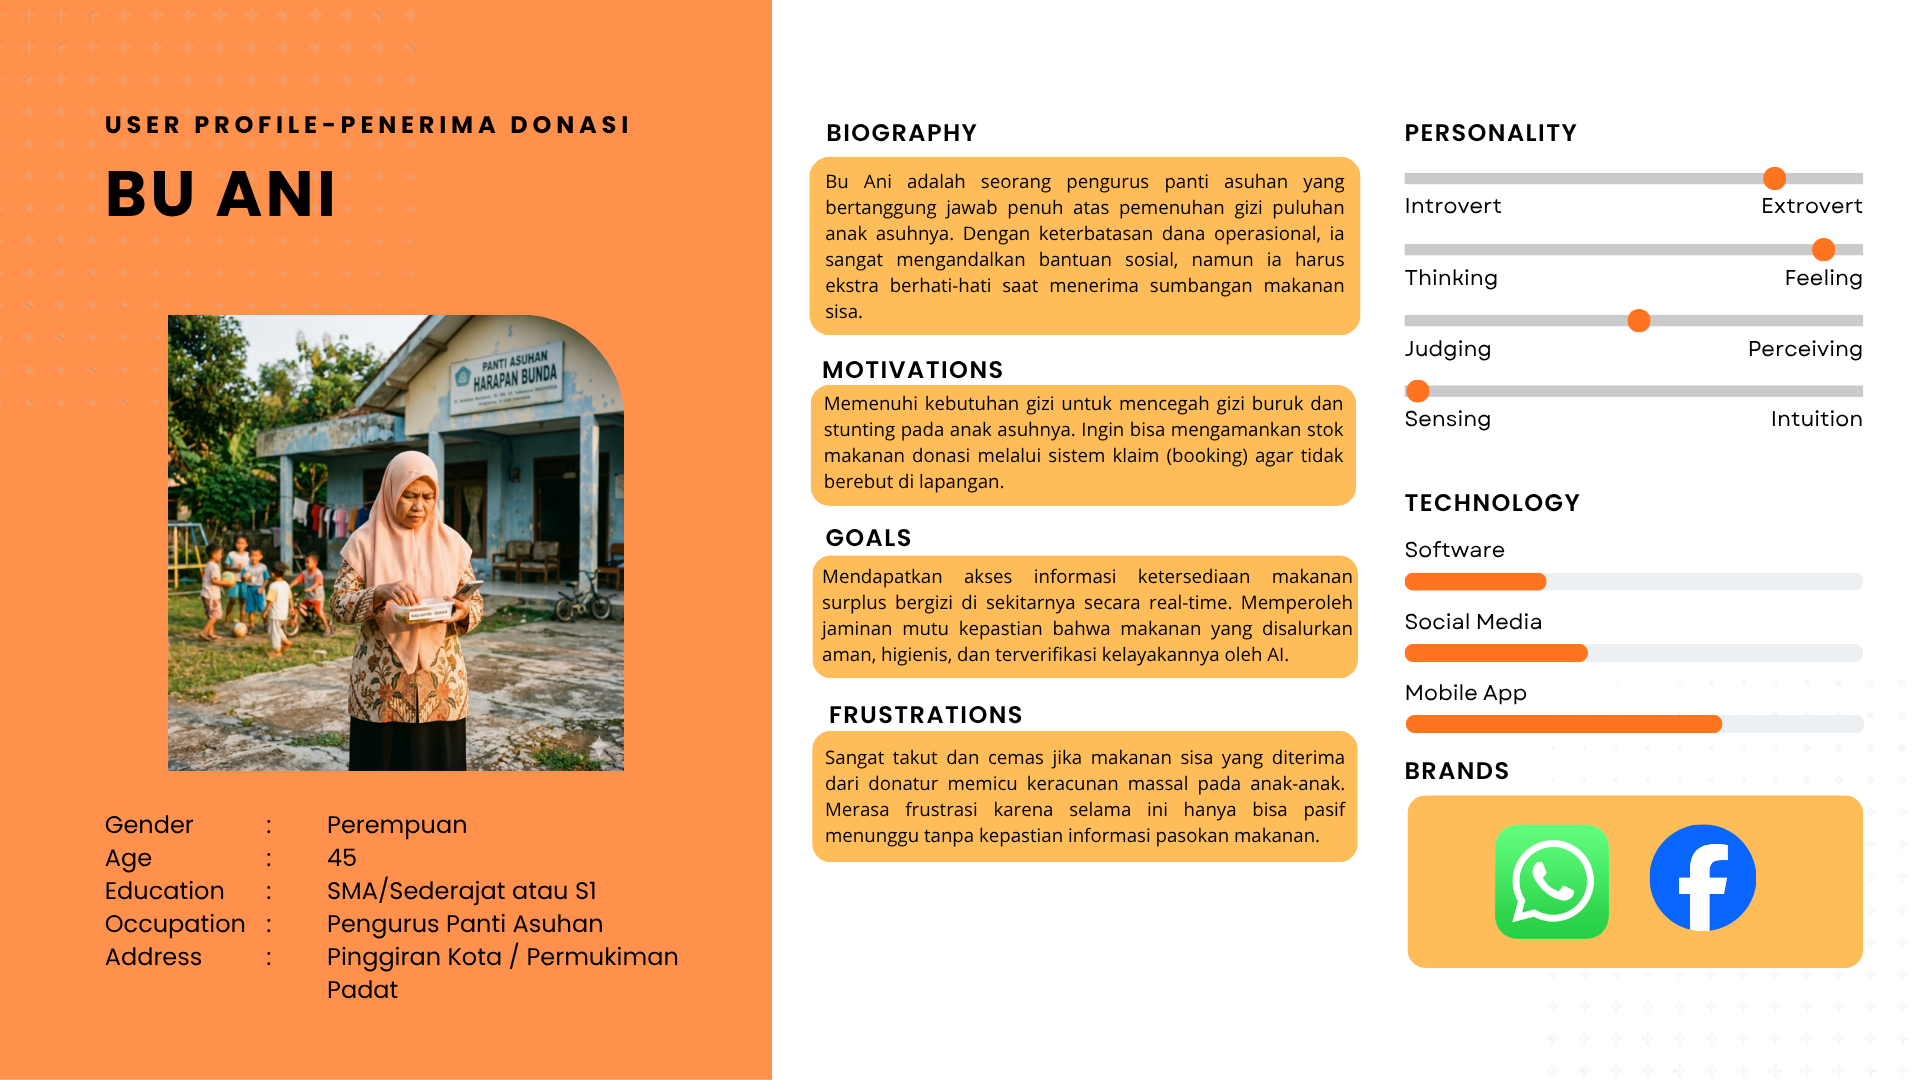
\includegraphics[width=1\textwidth]{image/bab2/segmentasi/UserPersona/Salinan dari baso arif/UP_PENERIMA DONASI.png}
    \caption{User Persona Penerima}
    \label{fig:userPersonaPenerima}
\end{figure}

Penjelasan Profil (Bu Ani):
Bu Ani (45 tahun) merupakan seorang pengurus panti asuhan di pinggiran kota/pemukiman padat. Ia memikul tanggung jawab penuh atas pemenuhan gizi puluhan anak asuhnya di tengah keterbatasan dana operasional.
\begin{itemize}
    \item Motivasi: Memenuhi kebutuhan gizi anak asuh demi mencegah kondisi gizi buruk dan \textit{stunting}. Ingin bisa mengamankan stok makanan donasi melalui sistem klaim (\textit{booking}) agar tidak perlu berebut di lapangan.
    \item Tujuan: Mendapatkan akses informasi terkait ketersediaan makanan surplus bergizi di sekitarnya secara \textit{real-time}, dengan jaminan mutu kepastian bahwa makanan tersebut aman, higienis, dan terverifikasi oleh AI.
    \item Frustrasi: Memiliki ketakutan mendalam jika makanan sisa yang diterima justru memicu keracunan massal pada anak-anak. Merasa frustrasi karena selama ini hanya bisa pasif menunggu bantuan tanpa kepastian pasokan.
    \item Preferensi: Aplikasi media sosial konvensional seperti WhatsApp dan Facebook.
\end{itemize}

\begin{figure}[H]
    \centering
    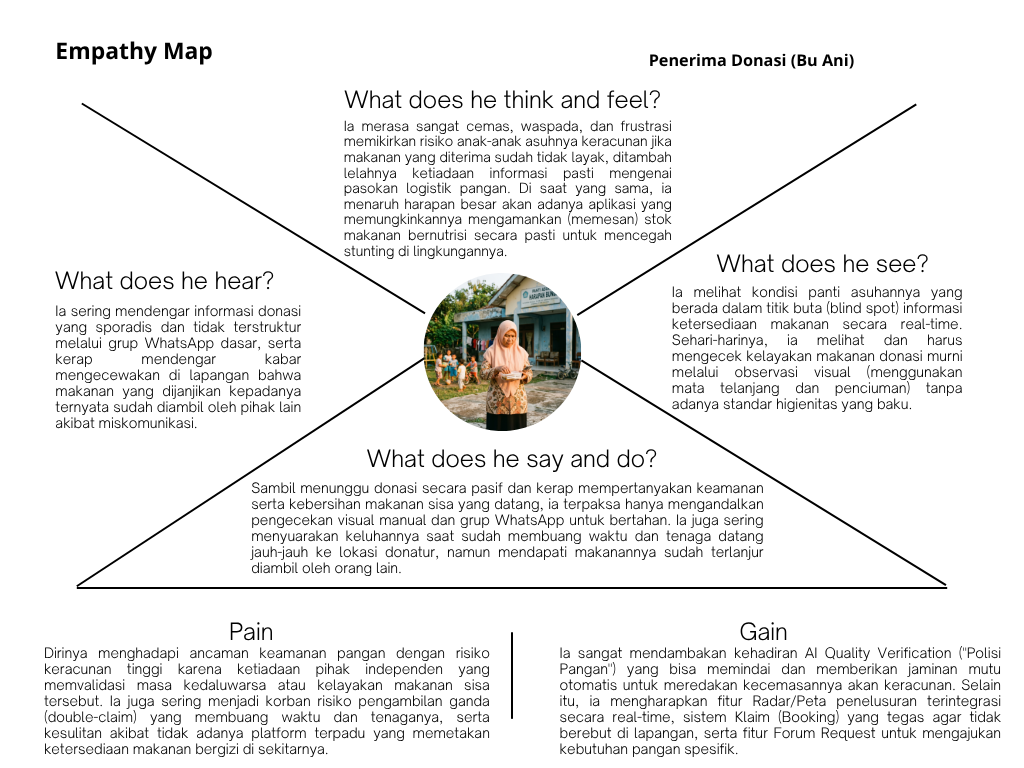
\includegraphics[width=1\textwidth]{image/bab2/segmentasi/EmpathyMap/Black and White Simple Empathy Map Brainstorm/EM_PENERIMA_DONASI.png}
    \caption{Empathy Map Penerima}
    \label{fig:empathyMapPenerima}
\end{figure}

Penjelasan Aspek Empathy Map (Bu Ani):
Bu Ani berada di pihak yang paling membutuhkan bantuan, namun juga pihak yang paling rentan terhadap risiko kesehatan dari makanan donasi.
\begin{itemize}
    \item THINKS \& FEELS: Merasa sangat cemas, waspada, dan didera frustrasi. Ia lelah dengan ketiadaan informasi pasti, ditambah memikirkan risiko anak asuhnya keracunan jika makanan yang diterima tidak layak. Ia menaruh harapan besar akan adanya aplikasi yang memungkinkannya mengamankan stok makanan bernutrisi secara pasti demi mencegah \textit{stunting}.
    \item HEARS: Kerap mendengar informasi donasi yang sporadis dan tidak terstruktur dari grup WhatsApp. Sayangnya, ia juga sering mendengar kabar mengecewakan di lapangan bahwa makanan yang dijanjikan sudah diambil oleh pihak lain akibat miskomunikasi.
    \item SEES: Menyadari kondisi panti asuhannya berada di titik buta (\textit{blind spot}) informasi ketersediaan makanan \textit{real-time}. Sehari-harinya, ia juga melihat dan harus mengecek kelayakan makanan murni melalui observasi visual manual (mata telanjang dan penciuman) tanpa standar higienitas baku.
    \item SAYS \& DOES: Sambil menunggu donasi secara pasif, ia hanya bisa mengandalkan pengecekan manual untuk bertahan. Ia kerap menyuarakan keluhan dan kekecewaannya saat sudah membuang tenaga dan waktu berjalan jauh, namun mendapati makanannya telah diambil orang lain.
    \item PAINS: Dirinya menghadapi ancaman keamanan pangan dengan risiko keracunan tinggi akibat ketiadaan alat validasi independen untuk makanan sisa. Ia sering menjadi korban perebutan/pengambilan ganda (\textit{double-claim}) yang membuang waktunya, serta kesulitan karena tidak ada platform peta terpadu ketersediaan makanan di sekitarnya.
    \item GAINS: Sangat mendambakan AI \textit{Quality Verification} ("Polisi Pangan") untuk menjamin mutu dan meredakan kecemasan akan keracunan. Ia juga mengharapkan fitur Peta Penelusuran \textit{real-time}, sistem Klaim (\textit{Booking}) agar tidak berebut di lapangan, serta Forum Request untuk mengajukan kebutuhan spesifik panti.
\end{itemize}

\begin{figure}[H]
    \centering
    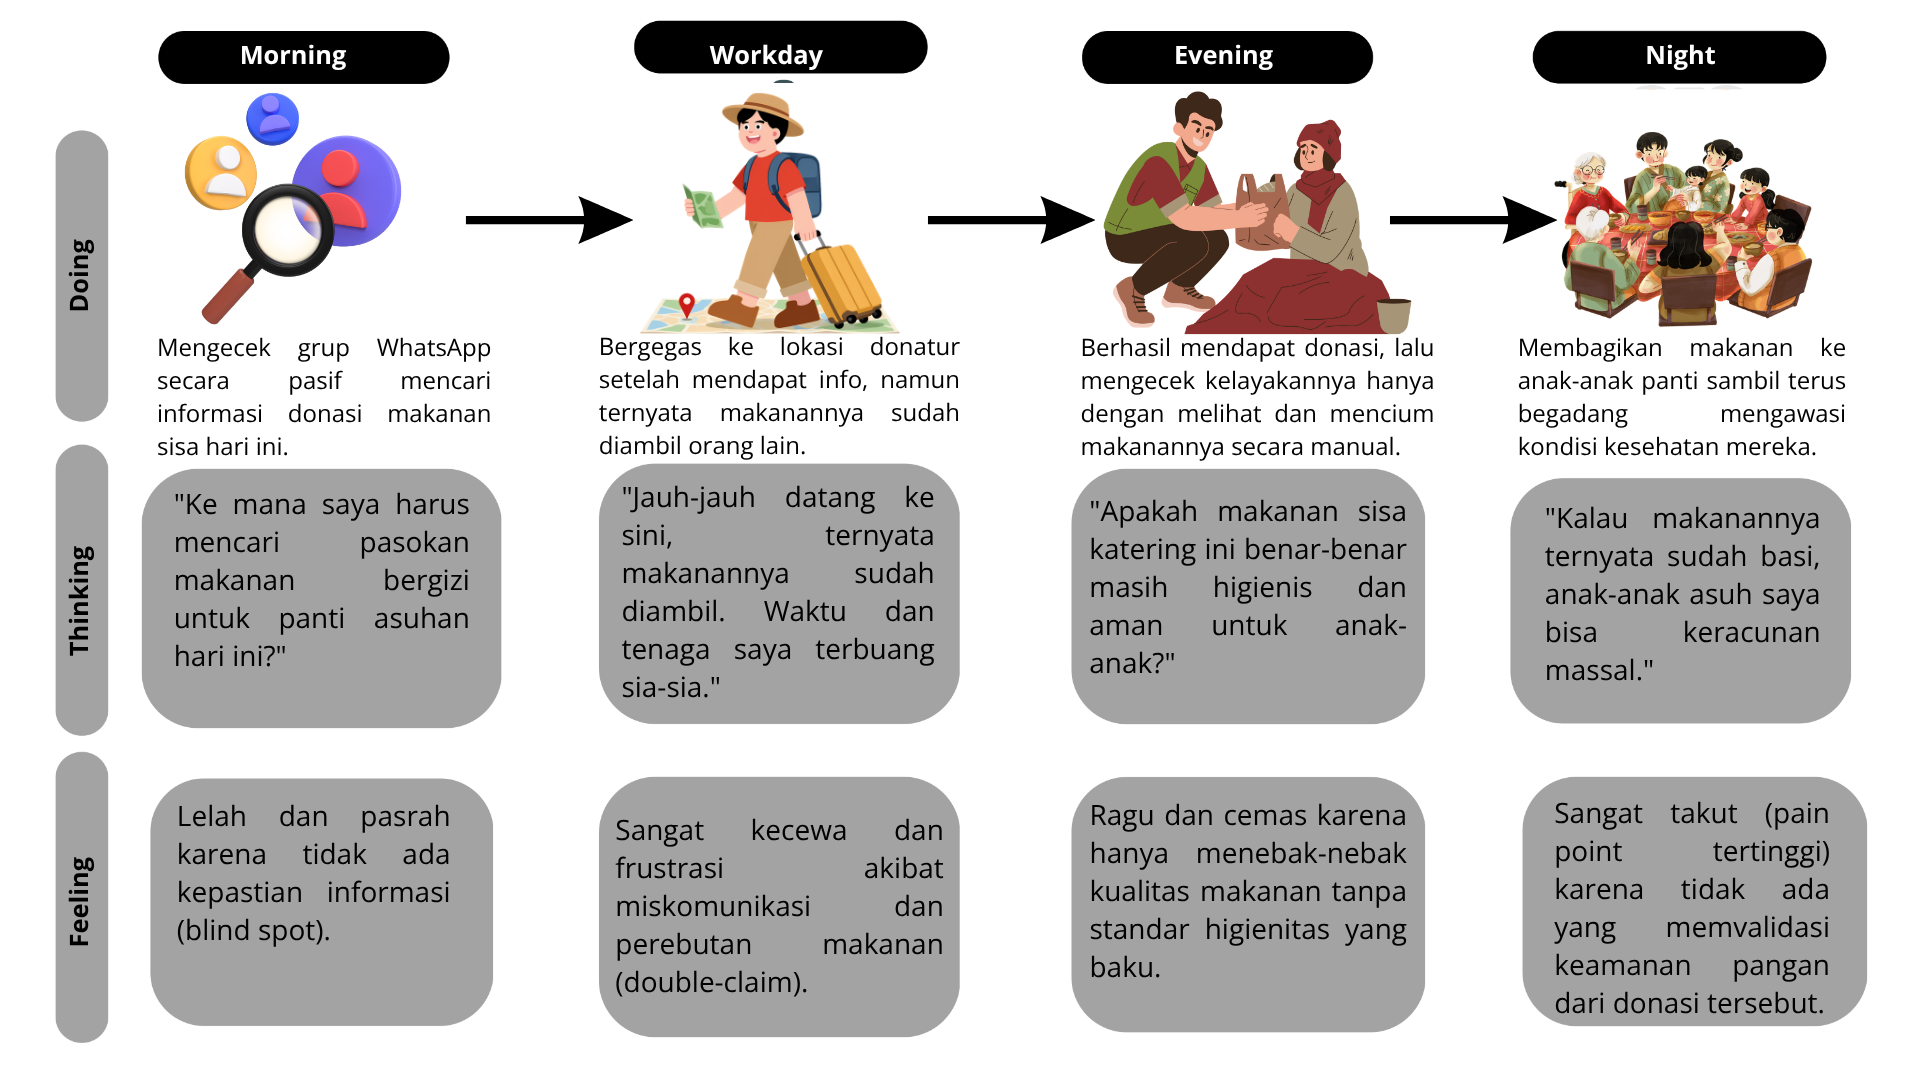
\includegraphics[width=0.99\textwidth]{image/bab2/segmentasi/CustomerJourneyMap/Salinan dari Template Journey Map/CJM_PENERIMA.png}
    \caption{Customer Journey Map Penerima}
    \label{fig:customerJourneyMapPenerima}
\end{figure}

Penjelasan Fase Customer Journey Map (Bu Ani): \\
\textit{Fase perjalanan: Pencarian Pasif $\rightarrow$ Pengejaran Donasi $\rightarrow$ Serah Terima Manual $\rightarrow$ Kekhawatiran Kesehatan}
\begin{description}
    \item[Pencarian Pasif (Pagi):] Bu Ani mengecek grup WhatsApp secara pasif untuk mencari informasi donasi makanan bergizi hari itu. Ia merasa lelah dan pasrah (\textit{Pain Points}) karena ketiadaan kepastian informasi (berada di \textit{blind spot}). Peluang Solusi (FAR): Fitur Peta Radar Penelusuran \textit{real-time} yang menampilkan ketersediaan donasi terdekat.
    \item[Pengejaran Donasi (Siang):] Bu Ani bergegas ke lokasi setelah mendapatkan info. Namun, ia sangat kecewa dan frustrasi (\textit{Pain Points}) karena makanannya ternyata sudah diambil orang lain akibat miskomunikasi dan perebutan makanan (\textit{double-claim}). Peluang Solusi (FAR): Fitur Sistem Klaim (\textit{Booking}) yang tegas sehingga makanan yang dipesan sudah "terkunci" untuknya.
    \item[Serah Terima Manual (Sore):] Ia akhirnya berhasil mendapat donasi. Namun, ia ragu dan cemas (\textit{Pain Points}) karena hanya bisa menebak-nebak kualitas makanan dengan melihat dan menciumnya tanpa adanya standar higienitas baku. Peluang Solusi (FAR): Proses verifikasi awal dari sisi donatur menggunakan AI \textit{Quality Verification}.
    \item[Kekhawatiran Kesehatan (Malam):] Bu Ani membagikan makanan ke anak-anak sambil begadang mengawasi kondisi mereka. Ia sangat takut (\textit{Pain Point Tertinggi}) bahwa kelalaiannya akan memicu keracunan massal karena tidak ada jaminan keamanan pangan. Peluang Solusi (FAR): Validasi "Polisi Pangan" yang memberi ketenangan batin (\textit{peace of mind}) secara mutlak.
\end{description}

% \clearpage

\begin{figure}[H]
    \centering
    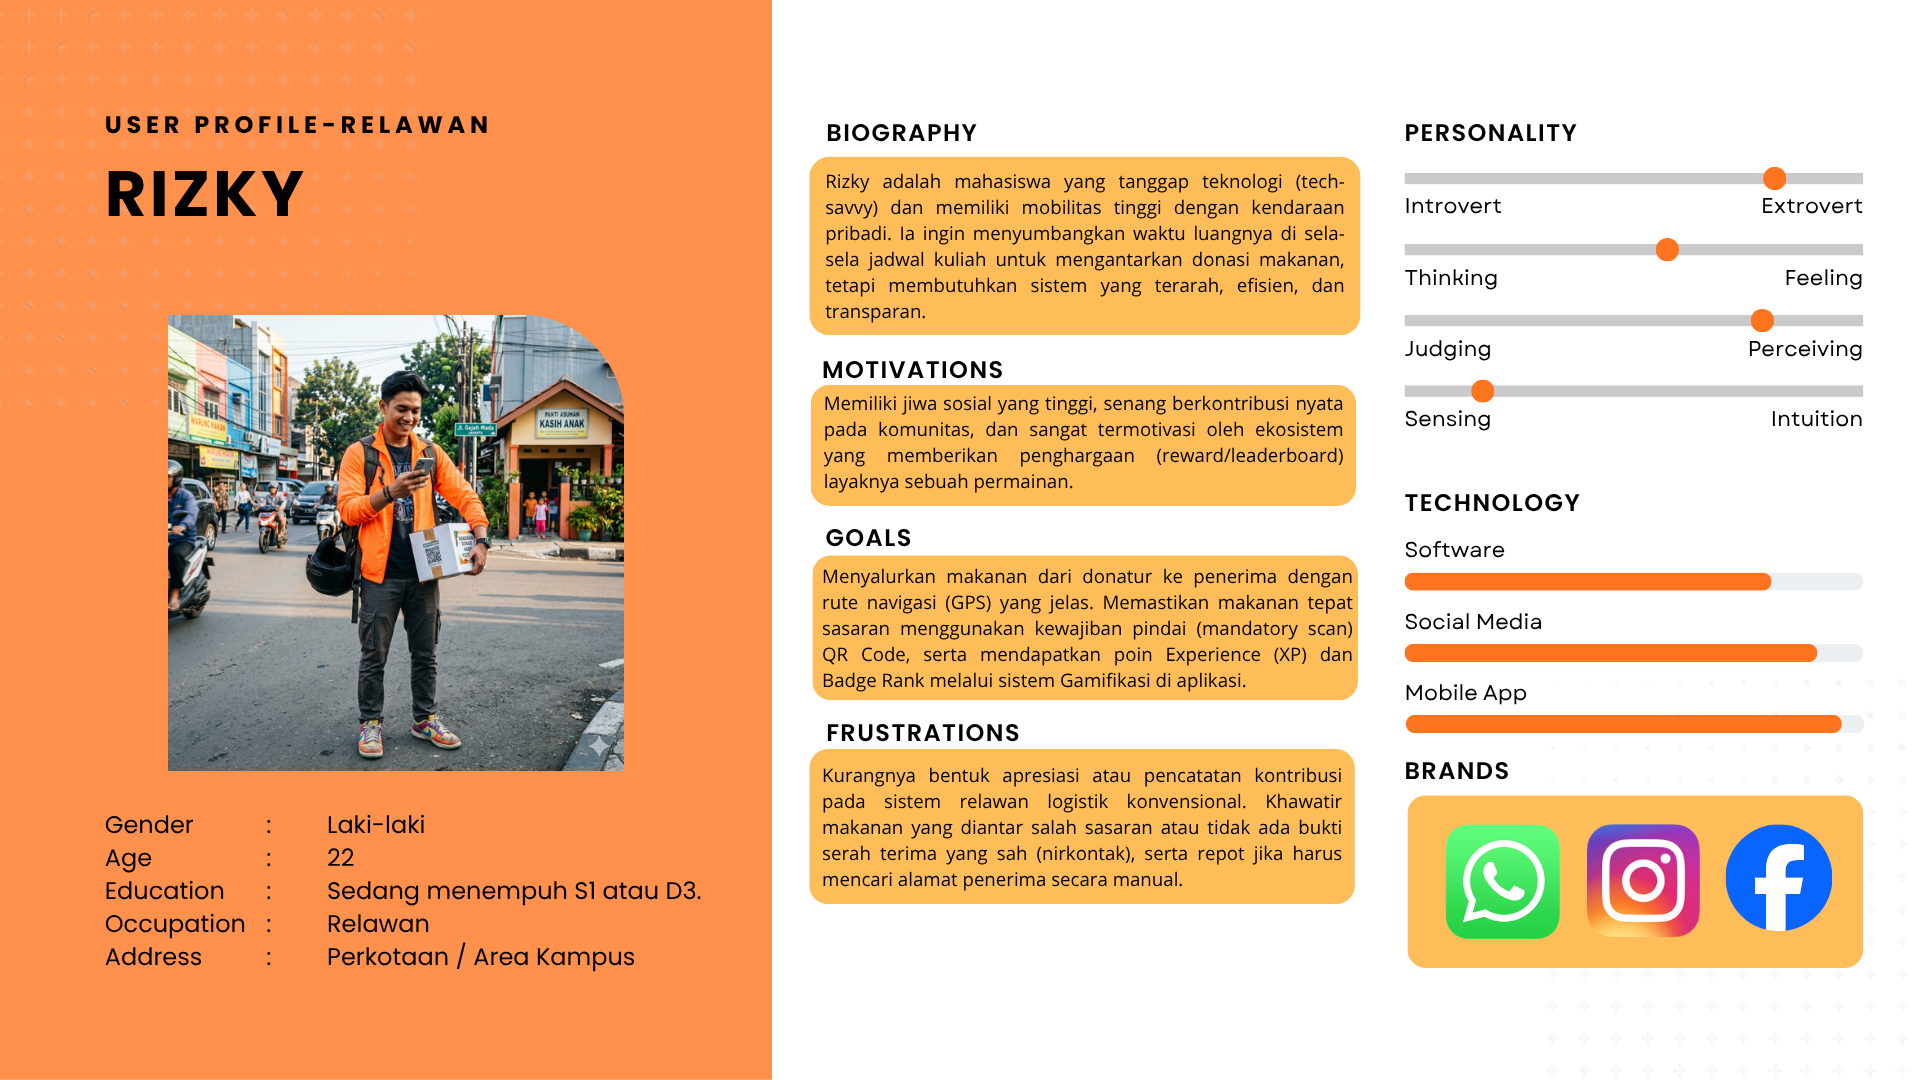
\includegraphics[width=1\textwidth]{image/bab2/segmentasi/UserPersona/Salinan dari baso arif/UP_RELAWAN.png}
    \caption{User Persona Relawan}
    \label{fig:userPersonaRelawan}
\end{figure}

Penjelasan Profil (Rizky):
Rizky (22 tahun) adalah seorang mahasiswa (\textit{tech-savvy}) dengan tingkat mobilitas tinggi menggunakan kendaraan pribadinya. Di sela-sela kepadatan jadwal kuliahnya, ia ingin menyumbangkan waktu luangnya untuk menjadi kurir logistik donasi makanan.
\begin{itemize}
    \item Motivasi: Memiliki jiwa sosial yang tinggi, senang berkontribusi nyata pada komunitas, dan sangat termotivasi oleh ekosistem yang memberikan penghargaan (\textit{reward/leaderboard}) layaknya sebuah permainan.
    \item Tujuan: Menyalurkan makanan dari donatur ke penerima menggunakan rute navigasi (GPS) yang jelas. Ia juga ingin memastikan makanan tepat sasaran menggunakan kewajiban pindai (\textit{mandatory scan}) QR Code, serta mendapatkan poin \textit{Experience} (XP) dan \textit{Badge Rank} melalui sistem gamifikasi.
    \item Frustrasi: Kurangnya bentuk apresiasi atau pencatatan kontribusi pada sistem relawan konvensional. Ia juga repot jika harus mencari alamat secara manual dan selalu khawatir makanan yang diantar salah sasaran tanpa adanya bukti serah terima yang sah.
    \item Preferensi: Aplikasi \textit{mobile}, perangkat lunak navigasi, media sosial, dan gamifikasi.
\end{itemize}

\begin{figure}[H]
    \centering
    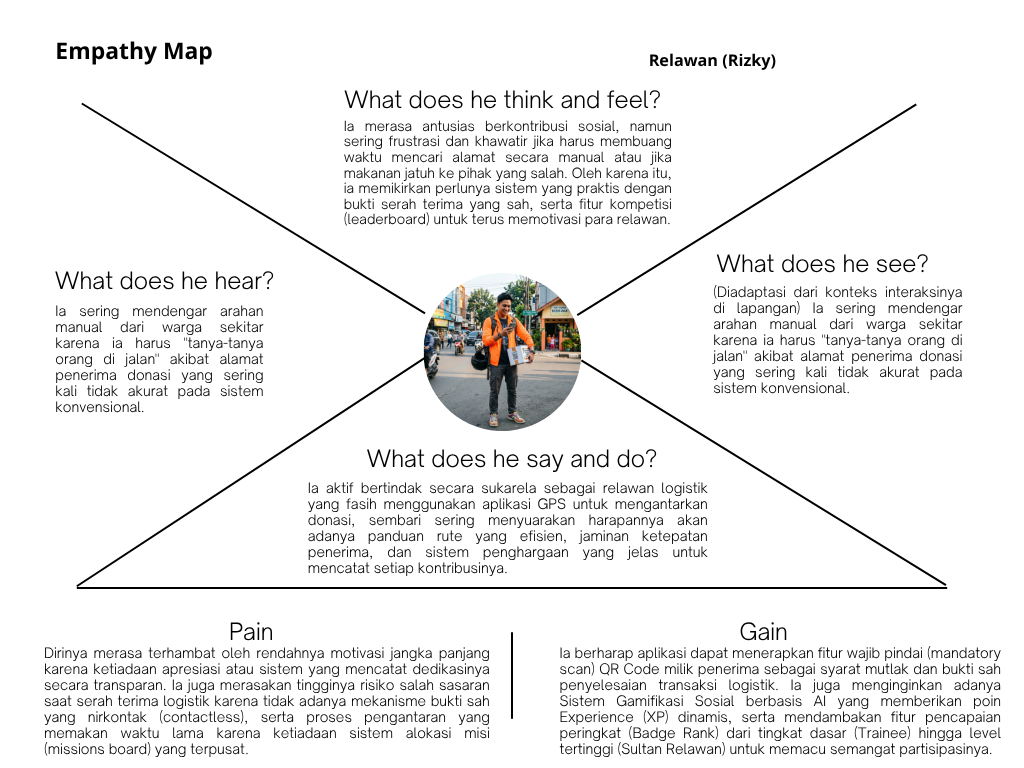
\includegraphics[width=1\textwidth]{image/bab2/segmentasi/EmpathyMap/Black and White Simple Empathy Map Brainstorm/EM_RELAWAN.png}
    \caption{Empathy Map Relawan}
    \label{fig:empathyMapRelawan}
\end{figure}

Penjelasan Aspek Empathy Map (Rizky):
Rizky merepresentasikan relawan muda yang bersemangat, namun kerap terhambat oleh inefisiensi sistem manual di lapangan.
\begin{itemize}
    \item THINKS \& FEELS: Merasa sangat antusias untuk berkontribusi sosial, namun sering dirundung frustrasi dan khawatir jika harus membuang waktu mencari alamat secara manual atau jika makanannya jatuh ke pihak yang salah. Ia memikirkan perlunya sistem praktis dengan bukti serah terima sah serta fitur kompetisi (\textit{leaderboard}) untuk memotivasinya.
    \item HEARS: Sering mendengar arahan manual dari warga sekitar karena ia harus "tanya-tanya orang di jalan" akibat titik alamat penerima donasi yang sering kali tidak akurat pada sistem konvensional.
    \item SEES: Dalam interaksinya di lapangan, ia melihat secara langsung betapa tidak akuratnya sistem alamat konvensional, sehingga ia berulang kali dihadapkan pada situasi harus mengandalkan arahan manual warga sekitar.
    \item SAYS \& DOES: Bertindak aktif secara sukarela sebagai relawan logistik yang fasih menggunakan aplikasi GPS. Sembari bekerja, ia sering menyuarakan harapannya akan adanya panduan rute efisien, jaminan ketepatan penerima, dan sistem penghargaan yang mencatat setiap kontribusinya.
    \item PAINS: Merasa terhambat oleh rendahnya motivasi jangka panjang akibat ketiadaan apresiasi dan pencatatan dedikasi transparan. Ia mengalami proses pengantaran yang memakan waktu lama karena ketiadaan sistem alokasi misi (\textit{missions board}) terpusat, serta tingginya risiko salah sasaran tanpa mekanisme bukti sah serah terima.
    \item GAINS: Berharap ada fitur Wajib Pindai (\textit{mandatory scan}) QR Code milik penerima sebagai syarat mutlak penyelesaian transaksi logistik. Ia juga sangat menginginkan Sistem Gamifikasi Sosial berbasis AI yang memberikan XP dinamis dan \textit{Badge Rank} (dari tingkat dasar/Trainee hingga Sultan Relawan).
\end{itemize}

\begin{figure}[H]
    \centering
    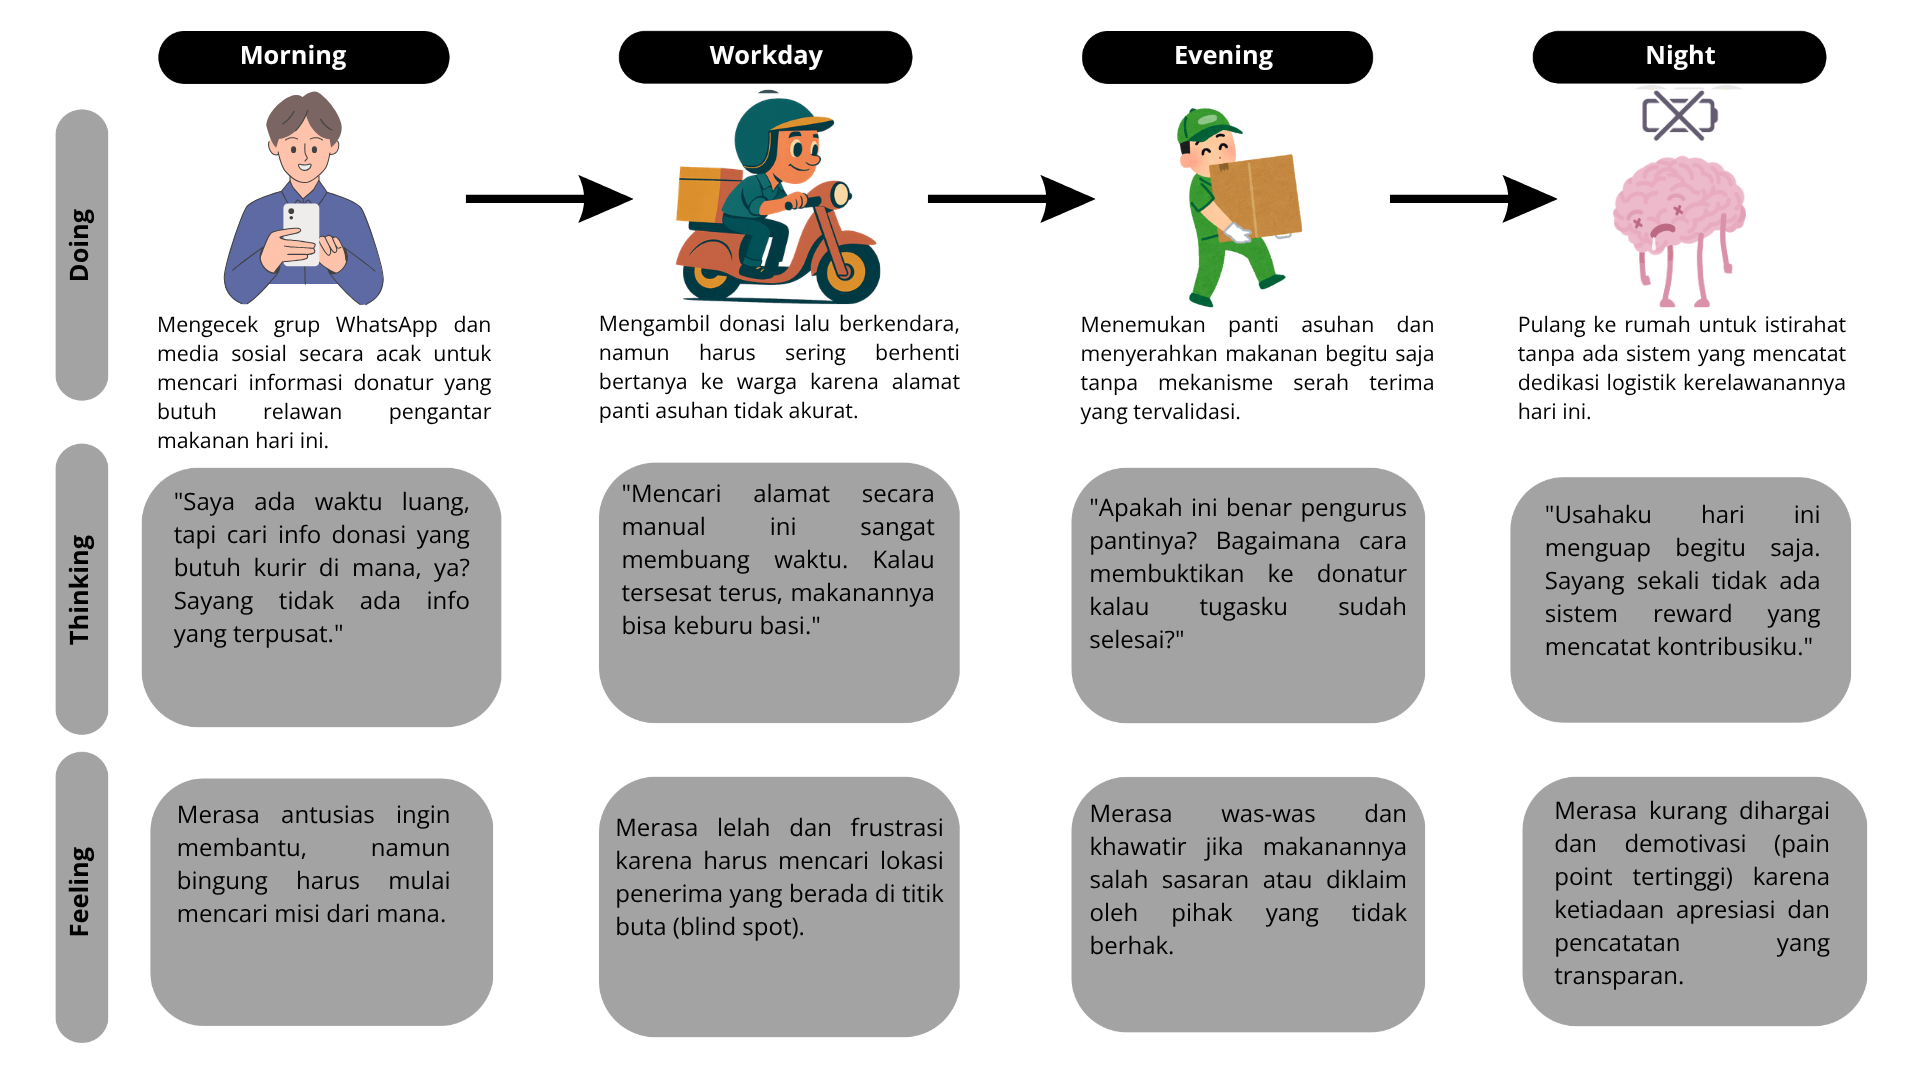
\includegraphics[width=0.85\textwidth]{image/bab2/segmentasi/CustomerJourneyMap/Salinan dari Template Journey Map/CJM_RELAWAN.png}
    \caption{Customer Journey Map Relawan}
    \label{fig:customerJourneyMapRelawan}
\end{figure}

Penjelasan Fase Customer Journey Map (Rizky): \\
\textit{Fase perjalanan: Pengecekan Misi $\rightarrow$ Penjemputan \& Pengantaran $\rightarrow$ Serah Terima Makanan $\rightarrow$ Pasca-Kerelawanan}
\begin{description}
    \item[Pengecekan Misi (Pagi):] Rizky memiliki waktu luang dan mengecek grup WhatsApp serta media sosial secara pasif untuk mencari donatur yang butuh kurir. Ia merasa antusias namun kebingungan (\textit{Pain Points}) karena informasi tidak terpusat. Peluang Solusi (FAR): Fitur \textit{Missions Board} terpusat yang menampilkan daftar penugasan logistik harian.
    \item[Penjemputan \& Pengantaran (Siang):] Rizky berkendara mengambil donasi, namun sering tersesat. Ia merasa lelah dan frustrasi (\textit{Pain Points}) karena mencari alamat manual di titik buta sangat membuang waktu dan berisiko membuat makanan keburu basi. Peluang Solusi (FAR): Navigasi GPS terintegrasi yang akurat menuju titik donatur dan penerima.
    \item[Serah Terima Makanan (Sore):] Rizky berhasil menemukan panti asuhan, namun merasa was-was dan khawatir (\textit{Pain Points}) menyerahkan makanan begitu saja karena tidak ada mekanisme validasi bahwa orang tersebut berhak menerimanya. Peluang Solusi (FAR): \textit{Mandatory Scan} QR Code nirkontak sebagai validasi serah terima yang mutlak.
    \item[Pasca-Kerelawanan (Malam):] Rizky pulang untuk istirahat. Ia merasa kurang dihargai dan sangat demotivasi (\textit{Pain Point Tertinggi}) karena dedikasi logistiknya menguap begitu saja tanpa ada sistem \textit{reward} atau pencatatan transparan. Peluang Solusi (FAR): Sistem Gamifikasi yang memberikan XP dan \textit{Badge Rank} seketika setelah misi selesai.
\end{description}
% \clearpage

\section{Identifikasi Aplikasi Sejenis}
\par Tahapan identifikasi aplikasi sejenis merupakan langkah analitis yang dilakukan untuk memetakan produk atau platform digital pendahulu (\textit{existing solutions}) yang memiliki kesamaan fungsional dengan sistem yang diusulkan. Tujuan utama dari observasi ini adalah untuk menemukan celah kelemahan (\textit{gap}) serta batasan operasional pada aplikasi yang telah beredar di masyarakat. Melalui analisis komparatif ini, pengembangan platform Food AI Rescue dapat difokuskan untuk merancang nilai tambah (\textit{value proposition}) yang lebih inovatif, tepat sasaran, dan relevan dalam menjembatani kebutuhan para pemangku kepentingan di ekosistem donasi pangan.

\par Dalam observasi ini, perbandingan difokuskan pada empat platform pengelola sisa makanan yang menjadi tolok ukur dalam inisiatif food rescue, yaitu:
\begin{enumerate}
    \item Surplus Indonesia: Aplikasi \textit{food rescue} komersial yang berfokus menyelamatkan makanan berlebih dari pelaku usaha (restoran, hotel, katering) dengan memfasilitasi pelanggan untuk membeli makanan yang belum habis terjual tersebut di akhir jam operasional dengan potongan harga hingga setengahnya.
    \item Garda Pangan: Organisasi \textit{food bank} di Indonesia yang berfokus pada penyelamatan surplus makanan dari industri \textit{hospitality} dan mendistribusikannya secara gratis kepada masyarakat pra-sejahtera melalui operasional jaringan relawan secara konvensional.
    \item Foodbank of Indonesia (FOI): Jaringan nirlaba nasional yang mengelola distribusi donasi dan makanan berlebih dari berbagai pihak untuk mencegah kelaparan, dengan fokus kampanye pada perbaikan gizi anak-anak balita dan kelompok rentan di berbagai wilayah.
    \item Too Good To Go: Aplikasi global pionir \textit{food rescue} (populer di Eropa dan Amerika) yang menghubungkan pelanggan dengan restoran atau toko kelontong untuk membeli ``paket kejutan'' (\textit{magic bags}) berisi makanan sisa layak konsumsi dengan harga yang sangat murah.
\end{enumerate}

\par Rincian perbandingan fitur dan kapabilitas layanan antara platform kompetitor dengan sistem Food AI Rescue yang diusulkan dapat diringkas pada tabel berikut:

\begin{table}[htbp]
    \centering
    \renewcommand{\arraystretch}{1.5}
    \caption{Perbandingan Fitur dan Kapabilitas Layanan Platform Food Rescue}
    \label{tab:perbandingan_fitur}
    \begin{tabularx}{\textwidth}{|L|C|C|C|C|C|}
        \hline
        \rowcolor{gray!10} Fitur / Layanan Utama & Surplus Indonesia & Garda Pangan & Foodbank of Indonesia & Too Good To Go & Food AI Rescue (Usulan) \\ \hline
        Penyaluran Donasi Makanan Secara Gratis & \xmark & \cmark & \cmark & \xmark & \cmark \\ \hline
        Verifikasi Kelayakan Makanan Otomatis (AI) & \xmark & \xmark & \xmark & \xmark & \cmark \\ \hline
        Sistem Penjemputan oleh Relawan Tergamifikasi & \xmark & \xmark & \xmark & \xmark & \cmark \\ \hline
        Validasi Serah Terima Nirkontak (QR Code) & \xmark & \xmark & \xmark & \xmark & \cmark \\ \hline
        Dasbor Kalkulasi Dampak Sosial (SROI) \textit{Real-Time} & \xmark & \xmark & \xmark & \xmark & \cmark \\ \hline
        Fitur AI Generatif untuk Kampanye CSR Korporat & \xmark & \xmark & \xmark & \xmark & \cmark \\ \hline
    \end{tabularx}
\end{table}

\newpage

\par Berdasarkan Tabel \ref{tab:perbandingan_fitur} di atas, dapat diidentifikasi beberapa celah (\textit{gap}) fungsionalitas yang menjadi landasan utama pengembangan Food AI Rescue. Platform komersial seperti Surplus Indonesia dan Too Good To Go sangat unggul dalam menyelamatkan sisa makanan dengan cepat, namun berfokus pada model transaksi jual-beli diskon, sehingga belum sepenuhnya menyasar masyarakat prasejahtera yang membutuhkan donasi secara cuma-cuma. Sementara itu, inisiatif sosial seperti Garda Pangan dan Foodbank of Indonesia memiliki rekam jejak penyaluran donasi gratis yang sangat baik, namun operasional logistiknya masih bersifat konvensional dan sangat bergantung pada verifikasi kelayakan makanan secara manual oleh manusia.

\par Lebih jauh lagi, keempat platform pembanding tersebut umumnya belum mengadopsi teknologi mutakhir seperti Kecerdasan Buatan (AI). Belum tersedia fitur otomatisasi yang mampu memverifikasi standar keamanan dan higienitas makanan secara visual (\textit{Computer Vision}), serta belum ada pelacakan metrik dampak lingkungan yang komprehensif. Platform pendahulu juga belum menyediakan dukungan fitur khusus yang memfasilitasi kebutuhan pelaporan donatur korporat dalam satu pusat kendali (\textit{dashboard}).

\par Oleh karena itu, usulan pengembangan Food AI Rescue hadir dengan posisi tawar (\textit{value proposition}) yang unik. Food AI Rescue menggabungkan penyaluran donasi pangan gratis, validasi keamanan berbasis AI (``Polisi Pangan''), dan operasional penjemputan logistik berbasis gamifikasi relawan ke dalam satu aplikasi yang ramah pengguna. Keberadaan Dasbor Dampak Sosial (SROI) \textit{real-time} serta pemisahan hak akses berbasis peran (\textit{Role-Based Access Control}) antara donatur, penerima, relawan, dan admin menjadikan platform ini tidak hanya sebagai alat penyalur bantuan teknis, tetapi juga sebagai ekosistem manajemen komunitas ketahanan pangan cerdas yang aman, transparan, dan terpadu.

\section{Analisis Kebutuhan Sistem}
Analisis persyaratan sistem merupakan langkah esensial dalam mentransformasikan kendala operasional pada sistem manual (As-Is) serta titik keluhan (pain points) para aktor lapangan ke dalam spesifikasi teknis yang komprehensif bagi platform Food AI Rescue. Tahapan analisis ini diklasifikasikan ke dalam tiga segmen utama, yakni pendefinisian tingkat hak akses pengguna (meliputi Donatur, Penerima, Relawan, Admin, dan SuperAdmin), pemetaan kebutuhan fungsional cerdas aplikasi, serta spesifikasi infrastruktur teknologi pendukung di sisi backend.

\subsection{Analisis Grup Akses}
\par Berdasarkan deskripsi pengguna dan pemetaan empati dari hasil rancangan \textit{User Persona}, terlihat jelas bahwa pengguna pada ekosistem aplikasi ini memiliki latar belakang literasi teknologi serta tanggung jawab operasional yang sangat bervariasi. Untuk mencegah pengguna awam kebingungan saat menavigasi fitur aplikasi, serta guna melindungi stabilitas infrastruktur sistem, seperti basis data dan konfigurasi Kecerdasan Buatan (AI), dari risiko penyalahgunaan atau kesalahan pengaturan (\textit{human error}), maka platform Food AI Rescue dirancang menggunakan arsitektur keamanan \textit{Role-Based Access Control} (RBAC).

\par Sistem ini membagi pengguna ke dalam 6 (enam) grup akses (\textit{role}) utama dengan pembatasan wewenang, fungsionalitas, dan pemanfaatan Kecerdasan Buatan (AI) yang sangat spesifik, yaitu:

\begin{enumerate}
    \item Donatur Individu
    \begin{itemize}
        \item Peranan: Pengguna dari kalangan masyarakat perorangan atau pelaku usaha skala mikro yang memiliki kelebihan produksi makanan layak konsumsi dalam jumlah kecil (skala rumah tangga).
        \item Hak Akses: Memiliki wewenang operasional untuk mengunggah data makanan surplus, memperbarui status ketersediaan (\textit{inventory}), dan melakukan serah terima donasi dengan wajib memindai Kode QR milik penerima sebagai bukti sah. Donatur individu juga berhak memantau Dasbor Dampak Sosial (SROI) secara langsung, serta menggunakan hak akses AI \textit{Quality Verification} (Polisi Pangan) untuk memvalidasi kelayakan makanan dan mendapatkan rekomendasi resep masakan.
    \end{itemize}

    \item Donatur Kelompok/Korporat (Mitra Penyedia)
    \begin{itemize}
        \item Peranan: Pengguna dari entitas bisnis skala besar, khususnya di sektor HORECA (Hotel, Restoran, dan Kafe), atau usaha katering berskala komersial yang menyumbangkan surplus makanan secara masif.
        \item Hak Akses: Memiliki wewenang manajemen distribusi dan pemantauan SROI yang sama dengan Donatur Individu. Sebagai nilai tambah untuk kebutuhan \textit{Corporate Social Responsibility} (CSR), peran ini dibekali hak akses AI Generatif eksklusif yang meliputi fitur \textit{Eco Packaging Editor} untuk merancang desain kemasan ramah lingkungan, dan fitur \textit{CSR Copywriter} untuk otomatisasi pembuatan naskah kampanye sosial.
    \end{itemize}

    \item Penerima (Mitra Penerima)
    \begin{itemize}
        \item Peranan: Kelompok masyarakat di kawasan rentan pangan, fasilitas sosial (seperti panti asuhan), dewan kemakmuran masjid (DKM), atau warga prasejahtera yang bertindak sebagai sasaran distribusi donasi.
        \item Hak Akses: Memiliki wewenang untuk mengakses radar peta (\textit{Map Dashboard}), mencari menu makanan terdekat, melakukan klaim (\textit{booking}) guna mencegah pengambilan ganda (\textit{double-claim}), dan menyajikan Kode QR miliknya untuk dipindai saat makanan tiba. Grup ini juga diberi hak untuk memberikan ulasan (\textit{feedback}), mengajukan permintaan spesifik via \textit{Forum Request}, serta menggunakan AI \textit{Quality Verification} untuk mengecek makanan sebelum dikonsumsi.
    \end{itemize}

    \item Relawan (Kurir)
    \begin{itemize}
        \item Peranan: Pengguna dari kalangan pemuda lokal atau masyarakat umum yang berpartisipasi secara sukarela (\textit{crowdsourcing}) sebagai armada penggerak logistik sosial penjemputan makanan.
        \item Hak Akses: Berwenang untuk mengakses daftar papan misi pengantaran, melakukan penjemputan makanan dari lokasi donatur, dan mengantarkannya ke titik lokasi penerima. Relawan memegang otoritas validasi lapangan dengan hak akses wajib pindai (\textit{mandatory scan}) Kode QR nirkontak sebagai syarat mutlak penyelesaian transaksi, yang secara otomatis terintegrasi dengan sistem poin gamifikasi (\textit{Leaderboard Ranking}).
    \end{itemize}

    \item Admin Pengelola
    \begin{itemize}
        \item Peranan: Tim manajerial dan pengawas operasional harian yang bertugas mengelola platform secara administratif di tingkat komunitas.
        \item Hak Akses: Memiliki wewenang administratif untuk memverifikasi pendaftaran akun baru, memblokir akun yang melakukan penyalahgunaan, menangani keluhan pengguna (\textit{support request}), serta memantau Dasbor Statistik (SROI) dan peta panas (\textit{heatmap}) sebaran donasi. Dari sisi kecerdasan buatan, Admin dibekali hak modifikasi panel \textit{Prompt Engineering} untuk menyesuaikan parameter instruksi deteksi AI secara \textit{real-time} tanpa perlu mengubah kode sumber aplikasi.
    \end{itemize}

    \item Super Admin
    \begin{itemize}
        \item Peranan: Pengguna dengan tingkat literasi teknologi tertinggi yang bertindak sebagai pengembang sistem (Tim IT / \textit{Programmer}) dan pemegang kedaulatan mutlak platform eksekutif.
        \item Hak Akses: Memiliki wewenang manajerial penuh terhadap operasional sistem di sisi peladen (\textit{backend}). Akses difokuskan pada manajemen tingkat makro seperti pemeliharaan server (\textit{Maintenance Mode}), perbaikan \textit{bug}, menjaga stabilitas basis data, mengelola pendaftaran akun Admin biasa, serta mengawasi hak prerogatif akses komputasi AI dan memonitor jejak \textit{log} sistem secara keseluruhan.
    \end{itemize}
\end{enumerate}

\subsection{Analisis Kebutuhan Fungsional}
Analisis kebutuhan fungsional menguraikan spesifikasi kapabilitas yang wajib dimiliki oleh sistem guna menjawab permasalahan pengguna di lapangan. Merujuk pada hasil observasi alur distribusi manual (As-Is) serta ekstraksi titik keluhan (\textit{pain points}) dari \textit{Empathy Map} dan \textit{User Journey Map}, platform yang dirancang harus mampu menghadirkan solusi berupa otomatisasi verifikasi kelayakan pangan berbasis Kecerdasan Buatan (AI), pencocokan donasi secara \textit{real-time}, serta rekapitulasi pelaporan dampak lingkungan (SROI) secara digital. Oleh karena itu, fungsionalitas yang akan diimplementasikan pada ekosistem Food AI Rescue diklasifikasikan ke dalam tujuh modul utama berikut:

\begin{enumerate}
    \item Kebutuhan Modul Autentikasi dan Manajemen Akun
    \begin{itemize}
        \item Sistem harus mampu memfasilitasi proses pendaftaran (\textit{register}) dan masuk (\textit{login}) yang keamanannya terenkripsi menggunakan algoritma sandi berlapis \textit{bcrypt}.
        \item Sistem harus memiliki pendeteksi perutean berbasis peran (\textit{Role-Based Router}) untuk mengarahkan pengguna secara spesifik ke antarmuka 6 (enam) grup akses yang berbeda (Donatur Individu, Donatur Korporat, Penerima, Relawan, Admin, dan SuperAdmin).
        \item Sistem harus menyediakan fitur manajemen profil pengguna, yang mencakup utilitas pemotongan gambar (\textit{crop image}) saat pengguna mengunggah foto \textit{avatar}.
    \end{itemize}

    \item Kebutuhan Modul Manajemen Donasi dan Inventori (Gudang Pangan)
    \begin{itemize}
        \item Sistem harus memfasilitasi pihak Donatur untuk membuat daftar donasi makanan baru beserta detail parameter minimum dan maksimum porsi yang tersedia.
        \item Sistem harus dilengkapi dengan manajemen inventori otomatis yang mampu menyembunyikan status tayangan donasi dari publik apabila batas waktu konsumsi (kedaluwarsa) telah terlewati.
        \item Sistem harus memfasilitasi donatur untuk melakukan validasi serah terima melalui fitur pemindaian Kode QR penerima secara nirkontak saat proses penyerahan berlangsung.
    \end{itemize}

    \item Kebutuhan Modul Integrasi Kecerdasan Buatan (AI)
    \begin{itemize}
        \item Sistem wajib terintegrasi dengan layanan \textit{Google Gemini Vision API} sebagai fitur ``Polisi Pangan'' untuk menjalankan verifikasi otomatis secara \textit{real-time}. AI harus mampu mendeteksi wujud makanan, menilai kelayakan konsumsi, higienitas visual, serta mengevaluasi kehalalan sebelum donasi diterbitkan.
        \item Sistem harus memfasilitasi fungsi bagi pengguna untuk memindai bahan sisa makanan guna mendapatkan rekomendasi resep masakan cerdas dari AI.
        \item Khusus bagi grup Donatur Korporat (HORECA), sistem harus menyediakan fitur AI Generatif eksklusif berupa \textit{Eco Packaging Editor} (didukung oleh Pollinations.ai) untuk merancang prototipe kemasan ramah lingkungan, serta asisten \textit{CSR Copywriter} untuk otomatisasi pembuatan naskah kampanye sosial.
    \end{itemize}

    \item Kebutuhan Modul Eksplorasi dan Klaim (Radar Penerima)
    \begin{itemize}
        \item Sistem harus menyediakan \textit{Map Dashboard} interaktif (memanfaatkan pustaka geolokasi \textit{Leaflet}) yang memungkinkan Mitra Penerima untuk melacak titik ketersediaan donasi pangan di sekitarnya.
        \item Sistem harus memungkinkan Penerima melakukan klaim (\textit{booking/checkout}) pesanan makanan untuk mencegah terjadinya insiden klaim ganda (\textit{double-claim}) oleh pihak lain pada stok yang sama.
        \item Sistem harus menyediakan \textit{Forum Request} yang memungkinkan Penerima untuk memublikasikan kebutuhan spesifik panti/fasilitas sosial mereka.
    \end{itemize}

    \item Kebutuhan Modul Operasional Logistik dan Gamifikasi (Relawan)
    \begin{itemize}
        \item Sistem harus menyediakan Papan Misi Penugasan (\textit{Missions Board}) yang merincikan titik penjemputan donatur dan titik serah terima akhir bagi armada Relawan.
        \item Sistem mewajibkan alur pemindaian silang (\textit{mandatory scan}) Kode QR menggunakan kamera aplikasi sebagai prasyarat mutlak verifikasi validitas penyelesaian distribusi logistik.
        \item Sistem harus dilengkapi mesin algoritma Gamifikasi (\textit{Leaderboard Ranking Engine}) yang secara otomatis memproses ketepatan waktu misi menjadi poin pengalaman (XP), lalu mengonversinya menjadi kasta peringkat atau medali sosial.
    \end{itemize}

    \item Kebutuhan Modul Pelacakan Dampak Sosial (SROI)
    \begin{itemize}
        \item Sistem harus memiliki Dasbor \textit{Sustainability Impact} terpadu yang merekapitulasi rekam jejak aktivitas donasi pengguna.
        \item Sistem harus memiliki kalkulator lingkungan yang mampu mengonversi kuantitas porsi makanan yang terselamatkan menjadi data analitik estimasi angka pengurangan emisi jejak karbon (kg CO$_2$) dan pelestarian air (liter).
    \end{itemize}

    \item Kebutuhan Modul Konfigurasi Pusat (Admin dan SuperAdmin)
    \begin{itemize}
        \item Sistem harus menyediakan \textit{Control Panel} operasional bagi Admin Pengelola untuk menindaklanjuti pendaftaran akun manual, membekukan akun yang melakukan pelanggaran, dan mengelola resolusi tiket keluhan pengguna melalui \textit{Support Request Manager}.
        \item Sistem harus menyediakan Dasbor Statistik Makro berupa peta panas (\textit{heatmap}) penyebaran donasi pangan.
        \item Sistem harus menyediakan instrumen khusus berupa panel \textit{Prompt Engineering Injection}. Panel ini memungkinkan Admin memodifikasi atau menajamkan parameter instruksi batas toleransi AI secara waktu nyata (\textit{real-time}) tanpa perlu mengubah kode sumber (\textit{source code}) aplikasi.
        \item Sistem harus memberi hak prerogatif (\textit{Maintenance Mode Trigger}) kepada SuperAdmin untuk mengendalikan penguncian server saat terjadi pemeliharaan, serta memantau rekam log (\textit{system logs}) seluruh aktivitas.
    \end{itemize}
\end{enumerate}

\subsection{Analisis Kebutuhan Dukungan Sistem}
Analisis kebutuhan dukungan sistem mendefinisikan seluruh infrastruktur teknis, baik dari segi perangkat lunak (\textit{software}), perangkat keras (\textit{hardware}), maupun konfigurasi lingkungan (\textit{environment}) yang disyaratkan agar platform Food AI Rescue (FAR) dapat beroperasi secara stabil. Mengingat platform ini dirancang menggunakan arsitektur \textit{Client-Server} yang terpisah antara \textit{Frontend} dan \textit{Backend}, maka spesifikasi dukungan sistemnya diuraikan ke dalam tiga kategori berikut:

\begin{enumerate}
    \item Kebutuhan Perangkat Lunak (\textit{Software})
    Untuk membangun dan menjalankan antarmuka (\textit{User Interface}) serta logika peladen (\textit{Server-Side}), sistem disyaratkan menggunakan tumpukan teknologi (\textit{tech stack}) terkini:
    \begin{itemize}
        \item Sisi Klien (\textit{Frontend}): Aplikasi antarmuka dibangun menggunakan \textit{framework} React.js (v19) yang dikombinasikan dengan TypeScript dan \textit{build tool} Vite agar dapat dieksekusi secara mulus pada \textit{web browser} (melalui antarmuka \texttt{localhost:5173}). Tampilan visual mengusung gaya \textit{Glassmorphism} interaktif, yang didukung oleh berbagai pustaka (\textit{library}) khusus seperti \texttt{react-leaflet} untuk pemetaan geolokasi, \texttt{react-easy-crop} untuk penyesuaian (\textit{cropping}) foto profil dan makanan, serta \texttt{lucide-react} untuk ikonografi.
        \item Sisi Server (\textit{Backend}): Logika sistem dan manajemen pangkalan data beroperasi dalam lingkungan (\textit{environment}) Node.js menggunakan \textit{framework} API Express.js (v5.x) pada antarmuka \texttt{localhost:5000}. Sistem basis data relasional dikelola menggunakan MySQL2 dengan skema \textit{database} utama \texttt{foodairescue}.
        \item Pustaka Modul Pendukung (\textit{Library}): Pada sisi \textit{backend}, sistem membutuhkan pustaka \texttt{bcryptjs} untuk perlindungan enkripsi kata sandi berlapis, \texttt{nodemailer} untuk layanan \textit{Simple Mail Protocol} (SMTP) notifikasi, serta \texttt{sharp} sebagai modul kompresi dan manipulasi gambar sebelum foto makanan dikirim ke jaringan AI.
        \item Layanan Pihak Ketiga (API AI): Sistem sangat bergantung pada \textit{Application Programming Interface} (API) eksternal, khususnya \textit{Google Gemini API} (\texttt{@google/genai} dan \texttt{@google/generative-ai}) sebagai inti intelijensi ``Polisi Pangan'', serta integrasi layanan \texttt{pollinations.ai} untuk mendukung fitur \textit{Eco Packaging Generator}.
    \end{itemize}

    \item Kebutuhan Perangkat Keras (\textit{Hardware})
    Karena pengembangan aplikasi Food AI Rescue pada fase iterasi awal (v1) ditujukan untuk pengujian lokal, maka dibutuhkan spesifikasi perangkat keras sebagai berikut:
    \begin{itemize}
        \item Perangkat Pengembang (\textit{Development}): Membutuhkan komputer personal (PC) atau laptop yang sepenuhnya mendukung \textit{Cross-Platform} (Windows, Mac OS, maupun Linux). Mesin pengembang harus mampu menjalankan \textit{local server} (seperti Apache dan MySQL melalui XAMPP/Laragon) serta mengeksekusi minimal dua terminal \textit{Command Node.js} secara serentak (untuk \textit{Frontend} dan \textit{Backend}).
        \item Perangkat Pengguna (Klien): Pengguna membutuhkan perangkat seluler pintar (\textit{smartphone}) atau komputer yang dilengkapi dengan koneksi internet yang stabil dan \textit{browser} modern. Khusus untuk Donatur, Penerima, dan Relawan, perangkat fisik wajib dilengkapi dengan fitur kamera yang berfungsi secara normal guna memfasilitasi pengambilan foto makanan donasi dan pemindaian wajib (\textit{mandatory scan}) Kode QR saat proses validasi serah terima.
    \end{itemize}

    \item Kebutuhan Konfigurasi Lingkungan (\textit{Environment Variables})
    \begin{itemize}
        \item Sistem Kredensial \texttt{.env}: Agar sistem dapat berjalan secara utuh, arsitektur FAR membutuhkan pengaturan rahasia berbasis \texttt{.env} pada \textit{root path} direktori proyek. Konfigurasi ini diwajibkan memuat parameter seperti \textit{port database}, URL pangkalan data, sandi akses \textit{localhost}, dan yang paling krusial adalah kunci rahasia eksekutif berupa \texttt{VITE\_GEMINI\_API\_KEY}. Tanpa adanya variabel kunci API ini terkonfigurasi dengan benar, sistem validasi cerdas dan keseluruhan pintu masuk aplikasi tidak akan merespon perintah.
    \end{itemize}
\end{enumerate}

% \\

\section{Analisis Kinerja Sistem}
Kinerja sistem merepresentasikan standar minimum dan tolok ukur (\textit{benchmark}) yang diterapkan guna memastikan seluruh ekosistem aplikasi Food AI Rescue, khususnya pada Modul Konfigurasi Pusat (Admin) dan Dasbor Dampak Sosial (SROI), mampu beroperasi selaras dengan spesifikasi dan perancangan fungsionalnya. Proses evaluasi kinerja dalam pengembangan platform ini dititikberatkan pada lima aspek utama, meliputi: fungsionalitas antarmuka perangkat lunak, keandalan serta stabilitas jalur komunikasi data (terutama integrasi \textit{Google Gemini API}), tingkat responsivitas keamanan sistem, efisiensi basis data, dan metrik kecepatan muat halaman (\textit{page load}). Ruang lingkup pengukuran kinerja ini tidak melibatkan pengujian ketahanan perangkat keras fisik (\textit{hardware}) di lapangan, melainkan dibatasi secara ketat pada domain rekayasa perangkat lunak dengan rincian standar pengujian sebagai berikut:

\begin{enumerate}
    \item Kinerja Waktu Respons dan Pemrosesan Media (\textit{Response Time \& Media Processing}) \\
    Mengingat sistem mengirimkan data visual ke server AI, kinerja waktu respons dijaga melalui optimalisasi \textit{payload} menggunakan pustaka \texttt{sharp}. Selain itu, penggunaan Vite pada React.js memastikan waktu muat halaman yang sangat cepat serta transisi antar-menu yang mulus.
    
    \item Kinerja Akurasi dan Keandalan AI (\textit{AI Accuracy \& Reliability}) \\
    Sistem dirancang tangguh untuk mitigasi bias deteksi (Anti-\textit{Clever Hans Effect}) agar AI tidak keliru menilai kelayakan makanan. Ketahanan terhadap manipulasi visual juga diperkuat melalui penajaman parameter \textit{Prompt Engineering} pada modul Admin.
    
    \item Kinerja Konkurensi dan Basis Data (\textit{Database Concurrency}) \\
    Pencegahan klaim ganda (\textit{double-claim prevention}) pada pangkalan data MySQL2 dilakukan melalui penanganan \textit{race-condition} secara \textit{real-time}, sehingga status inventaris dapat diperbarui dalam hitungan milidetik setelah permintaan divalidasi.
    
    \item Kinerja Keamanan dan Validasi Lapangan (\textit{Security \& Validation}) \\
    Keamanan data dijamin melalui enkripsi \texttt{bcryptjs} sebelum disimpan. Untuk validasi lapangan, sistem menggunakan mekanisme wajib pindai (\textit{mandatory scan}) Kode QR yang merespon secara instan guna memperbarui status penyelesaian transaksi.
    
    \item Kinerja Komputasi Analitik dan Gamifikasi (\textit{Analytical Efficiency}) \\
    Sistem melakukan kalkulasi dinamis SROI untuk menghitung pengurangan emisi karbon (CO$_2$) dan penghematan air secara \textit{real-time}. Algoritma \textit{Leaderboard Ranking} juga bekerja efisien di latar belakang untuk distribusi poin pengalaman (XP) relawan.
\end{enumerate}